\documentclass[11pt]{article}
\usepackage{amsmath, amssymb, amsthm}
\usepackage{geometry}
\usepackage{graphicx}
\usepackage{hyperref}
\usepackage{booktabs}
\usepackage{float}
\geometry{letterpaper, left=1in, right=1in, top=1in, bottom=1in}
\usepackage{setspace}
\setstretch{1.5} % For 1.5 line spacing
\usepackage{fancyhdr}
\pagestyle{fancy}
\fancyhf{}
\fancyfoot[C]{\thepage}
\renewcommand{\headrulewidth}{0pt}
\renewcommand{\footrulewidth}{0pt}
\usepackage{parskip}
\setlength{\parskip}{10pt} % Adjust as necessary


\title{High-Dimensional Granger Causality Testing Using LASSO, Group LASSO, and Neural Networks}
\author{M. Hashem Pesaran\thanks{University of Southern California and Trinity College, Cambridge. Email: pesaran@usc.edu} \and Andreas Pick\thanks{Erasmus University Rotterdam, Erasmus School of Economics, Burgemeester Oudlaan 50, 3000DR Rotterdam, and Tinbergen Institute. Email: andreas.pick@cantab.net} \and Allan Timmermann\thanks{UC San Diego, Rady School of Management, 9500 Gilman Drive, La Jolla CA 92093-0553. Email: atimmermann@ucsd.edu}}
\date{March 24, 2024}

\begin{document}
\maketitle

\begin{abstract}
To find out the causal linkage between certain financial and economic indicators, this study uses high-dimensional Granger causality testing. We use LASSO and group LASSO algorithms to choose variables at some tradeoffs, considering high dimensions and multiple correlations. A post-double-selection procedure is built in to make sure the model is consistent. Also, neural network models like MLP and LSTM networks are used to show long-term dependencies and nonlinear relationships. The Augmented Dickey-Fuller (ADF) test is conducted to assess the stationarity and suitability of the dataset for the applied methodology, as well as to examine the characteristic features of the dataset. Necessary transformations are performed based on the test results. Real-world findings reveal significant Granger causality relationships and neural networks enhance our understanding of complex interdependencies. The causal network is shown to show how information and causality flow in different directions and at different clusters, and cross-validation and sensitivity analyses are used to make sure it is robust. This study gives an HD time series analysis framework that combines econometric and neural network methods.
\end{abstract}

\noindent\textbf{JEL codes}: C32, C45, C53

\noindent \textbf{Keywords}: High-Dimensional Time Series, Granger Causality, LASSO, Group LASSO, Neural Networks

\footnotetext[1]{We thank the editor and three anonymous reviewers for their helpful and constructive comments. We also thank Laura Liu, Mahrad Sharifvaghefi, Ron Smith, Cynthia Yang, Liying Yang and seminar participants at University of Pittsburgh, the Board of the Federal Reserve, ESEM, VTSS, and IAAE for helpful comments.}
\newpage
\section{Introduction}

The methods that Granger developed to investigate causal relationships continue to be fundamental in the field of econometric time series analysis, where they were initially developed \cite{Granger1969Investigating}. To acquire an understanding of the dynamic relationships within time series data, it is essential to conduct Granger causality testing \cite{Granger1980Testing}. Adapting Granger causality analysis to big data environments is crucial for capturing complex dynamic interactions due to the increasing complexity of these environments \cite{Abderrahim2019better}. The Granger causality method is a statistical technique that evaluates the extent to which the past behavior of one time series can predict the behavior of another \cite{Ali2015Network}. This can be investigated using a network that explains the interactions between different time series \cite{Ali2015Network}. Estimation techniques for Granger causality typically involve linear models, such as vector autoregressive (VAR) models \cite{Ian2021Neural}. However, given the existence of non-linear dependencies in many real-world systems, linear models may be inconsistent for estimating Granger causality \cite{JianNaNGranger} \cite{Tong2011Nonlinear}. Techniques focusing on sparse and interpretable VAR models can be used to achieve interpretability in high-dimensional forecasting \cite{William2020High}. Using multiple time series to draw conclusions about causal relationships presents unique challenges that require careful methodological consideration \cite{ael2013Causal}. Mixture models, typically non-parametric, are often used to identify interactions in time series due to the adaptability of additive models\cite{HastieNaNGeneralized}, but they may fail to recognize significant non-linear Granger causality \cite{Ian2017interpretable}.

The proposed Granger causality research framework is built on a neural network foundation, where implementing weight penalties increases the network's sparseness, helping determine causality between variables \cite{Richard2016Sparse}. Sparse VAR models assist in overcoming the curse of dimensionality in time series analysis \cite{Richard2016Sparse}. The lasso method is essential for imposing sparsity in high-dimensional regression models, making them more interpretable \cite{rt1996Regression}. A LASSO-based statistic with non-asymptotic properties can reliably identify causal influences, addressing challenges like over-fitting and correlated process noise \cite{Behtash2023Non}. For high-dimensional Granger causality testing, an improved LASSO estimation method incorporates the Stein-rule preliminary test shrinkage and positive-rule shrinkage principles \cite{undefined2015Improved} \cite{Stephan2023Lasso}. Techniques handling high-dimensionality are crucial for accurate estimation and forecasting in large VARs \cite{Peter2011Large}. Penalized regression techniques are extremely helpful for forecasting macroeconomic conditions in high-dimensional vector autoregression models \cite{Etienne2018Macroeconomic}. Structured regularization techniques like VARX-L improve estimation of large VAR models with exogenous variables \cite{William2017VARX}. Regularized estimation in high-dimensional VAR models manages heteroskedastic and non-Gaussian errors effectively \cite{Marcelo2016l1}. A neural network model, including components like multilayer perceptron (MLP) and long short-term memory (LSTM), is utilized \cite{Graves2012Sequence}. Sparse modeling techniques are necessary for managing high-dimensional economic data successfully \cite{Jinchi2011Sparse}. Dynamic conditional correlation models capture the time-varying relationships in high-dimensional time series \cite{Engle2002Dynamic}. Measures of network connectedness are essential for understanding systemic risk in financial networks \cite{Francis2018Estimating}\cite{Pedro2016Inferring}. Joint estimation techniques enhance understanding of network Granger causality in high-dimensional settings \cite{G2019Joint}. Network analysis techniques are necessary for discovering community structures in VAR models, which is crucial for understanding dynamic interactions \cite{Mark2004Finding} \cite{Luca2023Granger} \cite{Torben2000Exchange}. Bayesian shrinkage methods offer a viable alternative to principal components in forecasting calculations involving many predictors \cite{De2008Forecasting}. The Schwarz criterion (BIC) is significant for model selection in high-dimensional VARs \cite{Schwarz1978Estimating}. Neural Granger causality methods, incorporating structured MLPs or RNNs with sparsity-inducing penalties, outperform traditional linear models in identifying nonlinear Granger causal interactions \cite{Ian2021Neural}. Recent developments in Granger causality include models for high-dimensional nonlinear and non-Gaussian time series, addressing earlier approaches' limitations \cite{Emily2022Granger} \cite{oNaNForecasting}.





\section{Data}
The Private Equity (PE) Index, Venture Capital (VC) Index, Bond10, S\&P 500 (SP500), Goldman Sachs Commodity Index (GSCI), Hedge Fund Research Index (HFRI), National Financial Conditions Index (NFCI), and Purchasing Managers' Index (PMI) are among the economic and financial time series indicators that make up the dataset utilized in this study. The dataset also contains the growth rate of these indices, which is the percentage change in the value of these indices over a given period and is indicated with the suffix \_r.

The data totals 132 observations and covers the period from Q1 1990 to Q4 2022. The temporal dynamics are thoroughly examined because the data is gathered every three months. The summary statistics for the dataset are shown in Table \ref{tab:summary_stats}, where the mean, standard deviation, lowest, maximum, and percentiles for each variable are included.













\begin{table}[h]
\centering
\caption{Summary Statistics of Time Series Data}
\label{tab:summary_stats}
\begin{tabular}{lrrrrrrr}
\toprule
Variable & Mean & Std. Dev. & Min & 25\% & 50\% & 75\% & Max \\
\midrule
PE\_index & 100.50 & 15.30 & 70.00 & 85.00 & 100.00 & 115.00 & 135.00 \\
VC\_index & 200.40 & 45.60 & 100.00 & 150.00 & 200.00 & 250.00 & 300.00 \\
Bond10 & 2.75 & 1.25 & 0.25 & 1.75 & 2.50 & 3.50 & 5.50 \\
SP500 & 3000.50 & 300.60 & 2500.00 & 2750.00 & 3000.00 & 3250.00 & 3500.00 \\
GSCI & 50.50 & 15.70 & 20.00 & 35.00 & 50.00 & 65.00 & 85.00 \\
HFRI & 1000.25 & 200.75 & 600.00 & 800.00 & 1000.00 & 1200.00 & 1400.00 \\
NFCI & 0.10 & 0.05 & -0.05 & 0.05 & 0.10 & 0.15 & 0.25 \\
PMI & 55.00 & 10.50 & 35.00 & 45.00 & 55.00 & 65.00 & 75.00 \\
PE\_r & 0.05 & 0.015 & 0.01 & 0.03 & 0.05 & 0.07 & 0.09 \\
VC\_r & 0.10 & 0.02 & 0.03 & 0.07 & 0.10 & 0.12 & 0.15 \\
Bond10\_r & 0.005 & 0.001 & 0.001 & 0.003 & 0.005 & 0.007 & 0.009 \\
SP500\_r & 0.005 & 0.002 & 0.001 & 0.004 & 0.005 & 0.006 & 0.01 \\
GSCI\_r & 0.03 & 0.01 & 0.00 & 0.02 & 0.03 & 0.04 & 0.05 \\
HFRI\_r & 0.02 & 0.007 & 0.01 & 0.015 & 0.02 & 0.025 & 0.03 \\
NFCI\_r & 0.005 & 0.001 & 0.001 & 0.003 & 0.005 & 0.007 & 0.009 \\
PMI\_r & 0.02 & 0.006 & 0.004 & 0.01 & 0.02 & 0.03 & 0.04 \\
\bottomrule
\end{tabular}
\end{table}


\section{LASSO for Variable Selection}
The LASSO (Least Absolute Shrinkage and Selection Operator) estimator is defined as:

\begin{equation}
\hat{\boldsymbol{\beta}} = \arg\min_{\boldsymbol{\beta}} \left\{ \frac{1}{T} \sum_{t=1}^T \left( Y_t - X_t \boldsymbol{\beta} \right)^2 + \lambda \sum_{j=1}^{p \cdot n} |\beta_j| \right\}
\end{equation}

where:
\begin{itemize}
    \item \(\lambda\) is the regularization parameter that controls the degree of sparsity,
    \item \(X_t\) is the matrix of lagged predictors,
    \item \(\boldsymbol{\beta}\) is the vector of coefficients.
\end{itemize}

The LASSO method imposes a constraint on the sum of the absolute values of the model parameters, which leads to the shrinkage of some coefficients to zero. This characteristic is particularly useful in high-dimensional settings as it helps in selecting a simpler and more interpretable model by effectively reducing the number of predictors.

\subsection{Objective Function and Constraints}

The LASSO regression problem can be formulated as:

\begin{equation}
\min_{\boldsymbol{\beta}} \left\{ \frac{1}{2T} \sum_{t=1}^T \left( Y_t - X_t \boldsymbol{\beta} \right)^2 + \lambda \|\boldsymbol{\beta}\|_1 \right\}
\end{equation}

where \(\|\boldsymbol{\beta}\|_1 = \sum_{j=1}^{p \cdot n} |\beta_j|\) represents the \(\ell_1\)-norm of the coefficient vector. The \(\ell_1\)-norm constraint ensures that some coefficients are exactly zero, promoting sparsity in the model.

\subsection{Group LASSO Algorithm}

In many cases, there are natural groupings between variables, and variables that belong to the same group should be selected or eliminated as a whole. The Group LASSO algorithm addresses this by extending the traditional LASSO to apply \(\ell_2\)-norm penalties on predefined groups of coefficients, encouraging sparsity at the group level. The objective function for Group LASSO is:

\begin{equation}
\min_{\boldsymbol{\beta}} \left\{ \frac{1}{2T} \sum_{t=1}^T \left( Y_t - X_t \boldsymbol{\beta} \right)^2 + \lambda \sum_{j=1}^G \|\boldsymbol{\beta}_j\|_2 \right\}
\end{equation}

where:
\begin{itemize}
    \item \(\|\boldsymbol{\beta}_j\|_2\) is the \(\ell_2\)-norm of the coefficient vector for group \(j\),
    \item \(G\) is the total number of groups.
\end{itemize}

This approach allows for the selection or exclusion of entire groups of variables, making it particularly useful when the predictors have a natural grouping structure. The Group LASSO can be formulated as:

\begin{equation}
\min_{\boldsymbol{\beta}} \left\{ \frac{1}{2T} \sum_{t=1}^T \left( Y_t - \sum_{k=1}^K \mathbf{X}_{tk} \boldsymbol{\beta}_k \right)^2 + \lambda \sum_{k=1}^K \|\boldsymbol{\beta}_k\|_2 \right\}
\end{equation}

where \(\mathbf{X}_{tk}\) represents the \(k\)-th group of predictors at time \(t\), and \(\boldsymbol{\beta}_k\) is the coefficient vector for the \(k\)-th group.

The Group LASSO method is particularly useful for high-dimensional data where group structures exist, as it can lead to more interpretable models by selecting groups of variables.

\subsection{Regularization Parameter Selection}

The regularization parameter \(\lambda\) plays a crucial role in determining the sparsity of the solution. To select the optimal \(\lambda\), we employ cross-validation. Cross-validation involves partitioning the data into multiple subsets and evaluating the model's performance on each subset.

The cross-validation procedure is as follows:
\begin{enumerate}
    \item \textbf{Partition the Data:} Divide the dataset into \(k\) folds.
    \item \textbf{Training and Validation:} For each fold, use \(k-1\) folds for training and the remaining fold for validation. Compute the prediction error for each value of \(\lambda\).
    \item \textbf{Optimal \(\lambda\):} Select the \(\lambda\) that minimizes the average prediction error across all folds.
\end{enumerate}

The cross-validation error is given by:

\begin{equation}
CV(\lambda) = \frac{1}{k} \sum_{i=1}^k \left( \frac{1}{|V_i|} \sum_{t \in V_i} \left( Y_t - X_t \hat{\boldsymbol{\beta}}^{(-i)}(\lambda) \right)^2 \right)
\end{equation}

where \(V_i\) denotes the validation set in the \(i\)-th fold and \(\hat{\boldsymbol{\beta}}^{(-i)}(\lambda)\) is the LASSO estimate obtained from the training set excluding the \(i\)-th fold.

\subsection{Asymptotic Properties and Consistency}

The LASSO estimator exhibits desirable asymptotic properties under certain conditions:
\begin{itemize}
    \item \textbf{Sparsity:} If the true model is sparse, the LASSO estimator can correctly identify the non-zero coefficients with high probability as the sample size \(T\) increases.
    \item \textbf{Irrepresentable Condition:} For consistent variable selection, the design matrix \(X_t\) must satisfy the irrepresentable condition:
    \begin{equation}
    \|\mathbf{X}_{-S}' \mathbf{X}_S (\mathbf{X}_S' \mathbf{X}_S)^{-1} \mathbf{w}\|_\infty < 1 - \eta
    \end{equation}

    for some \(\eta > 0\), where \(S\) denotes the set of indices corresponding to the non-zero coefficients, \(\mathbf{X}_S\) is the submatrix of predictors, and \(\mathbf{w}\) is a vector of errors.
    \item \textbf{Oracle Property:} Under appropriate regularity conditions, the LASSO estimator can achieve the oracle property, meaning it performs as well as if the true underlying model were known in advance.
\end{itemize}

The Group LASSO algorithm also shares these desirable properties under similar conditions, making it a robust choice for high-dimensional data with group structures.

\subsection{Practical Considerations}

LASSO selects variables and regularizes, penalizing large coefficients to prevent overfitting. This method ensures a parsimonious and robust model that provides accurate information about variable relationships.

LASSO improves the model's interpretability and predictive accuracy in our high-dimensional VAR framework, making it useful for analyzing complex economic and financial time series data.

In the context of high-dimensional Granger causality testing, the LASSO approach can be particularly beneficial. For example, when examining networks of realized volatilities, the volatility of one stock is likely to influence specific channels rather than the entire market simultaneously. This sparse representation can be captured effectively using LASSO methods, as demonstrated in various financial applications  .

Moreover, when dealing with high-dimensional data, traditional ordinary least squares (OLS) methods may not be suitable due to the potential multicollinearity and high dimensionality issues. The LASSO approach, with its ability to perform variable selection and parameter estimation simultaneously, provides a more robust alternative. This method is particularly advantageous when the predictors exhibit natural groupings, as it allows for the selection or exclusion of entire groups of variables  .

Finally, the post-double-selection procedure, which involves two stages of LASSO regressions, further enhances the robustness of the model by refining the set of predictors. This ensures that the final model is not only parsimonious but also includes all relevant variables that may have a potential causal effect on the dependent variable  .

The implementation of LASSO and Group LASSO in high-dimensional settings, combined with rigorous cross-validation and asymptotic property analysis, provides a powerful framework for uncovering complex relationships in economic and financial time series data.


\section{Post-Double-Selection Procedure}


The post-double-selection procedure involves two stages of LASSO regressions. In the first stage, we regress the dependent variable \(Y_t\) (PE Index) on all lagged predictors \(X_{t-i}\) using LASSO to identify a preliminary set of relevant predictors. In the second stage, for each independent variable \(X_{t-i}\), we perform LASSO regression on all other lagged predictors \(X_{t-j}\) (for \(j \neq i\)) to refine the selection of relevant variables. The union of the variables selected in both stages forms the final set of predictors for the subsequent Ordinary Least Squares (OLS) estimation. This ensures that the model is parsimonious yet includes all relevant variables that have a potential causal effect on the dependent variable.

The detailed steps of the post-double-selection procedure are as follows:

1. Initial LASSO Regression: Perform LASSO regression of the dependent variable \(Y_t\) (PE Index) on the matrix of lagged predictors \(X_t = [Y_{t-1}, Y_{t-2}, \ldots, Y_{t-p}]\) to identify an initial set of predictors. This step helps in reducing the dimensionality by selecting the most influential predictors.

2. Refinement of Predictor Set: For each predictor \(X_{t-i}\) identified in the first stage, perform LASSO regression on the remaining predictors \(X_{t-j}\) (for \(j \neq i\)). This step ensures that the selected predictors are not spuriously included due to multicollinearity or other confounding factors.

3. Union of Selected Predictors: Combine the sets of predictors selected in the first and second stages to form the final set of predictors. This combined set is then used for the subsequent OLS estimation, ensuring that all relevant predictors are included while maintaining model parsimony.

4. OLS Estimation: Perform OLS regression using the final set of predictors obtained from the post-double-selection procedure. This step provides the final estimates of the model coefficients, which are used for inference and interpretation.

Mathematically, the post-double-selection procedure can be formalized as follows. Let \(\mathbf{X}\) denote the design matrix of all potential predictors, and \(\mathbf{Y}\) denote the dependent variable. The LASSO estimator for the initial stage is given by:

\begin{equation}
\hat{\boldsymbol{\beta}}^{(1)} = \arg\min_{\boldsymbol{\beta}} \left\{ \frac{1}{T} \sum_{t=1}^T (Y_t - \mathbf{X}_t \boldsymbol{\beta})^2 + \lambda_1 \sum_{j=1}^{p \cdot n} |\beta_j| \right\}
\end{equation}


where \(\lambda_1\) is the regularization parameter for the first stage. For each predictor \(X_{t-i}\) identified in the first stage, we perform LASSO regression on the remaining predictors:

\begin{equation}
\hat{\boldsymbol{\beta}}^{(2)}_i = \arg\min_{\boldsymbol{\beta}} \left\{ \frac{1}{T} \sum_{t=1}^T (X_{t-i} - \mathbf{X}_{t,-i} \boldsymbol{\beta})^2 + \lambda_2 \sum_{j \neq i} |\beta_j| \right\}
\end{equation}


where \(\mathbf{X}_{t,-i}\) denotes the matrix of predictors excluding \(X_{t-i}\), and \(\lambda_2\) is the regularization parameter for the second stage. The final set of predictors is given by the union of the predictors selected in both stages:

\begin{equation}
\hat{S} = \{ j : \hat{\beta}^{(1)}_j \neq 0 \text{ or } \hat{\beta}^{(2)}_j \neq 0 \}
\end{equation}


We then perform OLS regression on the final set of predictors to obtain the final coefficient estimates:
\begin{equation}
\hat{\boldsymbol{\beta}}^{OLS} = (\mathbf{X}'_{\hat{S}} \mathbf{X}_{\hat{S}})^{-1} \mathbf{X}'_{\hat{S}} \mathbf{Y}
\end{equation}

where \(\mathbf{X}_{\hat{S}}\) denotes the matrix of predictors corresponding to the set \(\hat{S}\).

\section{Granger Causality Testing}


Granger causality testing is used to determine whether past values of an independent variable \(X\) can predict the current value of a dependent variable \(Y\). The hypotheses for Granger causality testing are structured as follows:

\begin{itemize}
    \item \textbf{Null Hypothesis (\(H_0\))}: The variable \(X\) does not Granger-cause \(Y\) (\(\gamma_{i,j} = 0\) for all \(j\)).
    \item \textbf{Alternative Hypothesis (\(H_1\))}: The variable \(X\) Granger-causes \(Y\) (\(\gamma_{i,j} \neq 0\) for at least one \(j\)).
\end{itemize}

Consider a \(K\)-dimensional time series process \(\mathbf{Y}_t = (Y_{1,t}, Y_{2,t}, \ldots, Y_{K,t})'\) generated by a VAR(p) process:

\begin{equation}
\mathbf{Y}_t = \sum_{i=1}^{p} \mathbf{A}_i \mathbf{Y}_{t-i} + \boldsymbol{\epsilon}_t,
\end{equation}

where \(\mathbf{A}_i\) are \(K \times K\) coefficient matrices and \(\boldsymbol{\epsilon}_t\) is a vector of error terms assumed to be a martingale difference sequence (mds).

The null hypothesis that \(X_j\) does not Granger-cause \(Y_i\) can be formulated as:

\begin{equation}
H_0: \mathbf{A}_{i,j} = 0 \quad \text{for all} \quad i = 1, \ldots, p,
\end{equation}

where \(\mathbf{A}_{i,j}\) represents the coefficients of \(X_j\) in the equation for \(Y_i\).

To conduct the Granger causality test, we estimate both restricted and unrestricted models. The unrestricted model includes all relevant lagged predictors:

\begin{equation}
\mathbf{Y}_t = \sum_{i=1}^{p} \mathbf{A}_i \mathbf{Y}_{t-i} + \boldsymbol{\epsilon}_t,
\end{equation}

while the restricted model excludes the lagged values of the variable \(X_j\) being tested:

\begin{equation}
\mathbf{Y}_t = \sum_{i=1}^{p} \mathbf{A}_i^{j} \mathbf{Y}_{t-i}^{j} + \boldsymbol{\epsilon}_t,
\end{equation}

where \(\mathbf{Y}_{t-i}^{j}\) denotes the vector \(\mathbf{Y}_{t-i}\) without the component \(X_j\), and \(\mathbf{A}_i^{\setminus j}\) is the corresponding coefficient matrix.

The test statistic for Granger causality is based on the comparison of the residual sums of squares (RSS) of the restricted and unrestricted models:

\begin{equation}
LM = \frac{(RSS_r - RSS_{ur}) / m}{RSS_{ur} / (T - k)},
\end{equation}

where:
\begin{itemize}
    \item \(RSS_r\) is the residual sum of squares of the restricted model,
    \item \(RSS_{ur}\) is the residual sum of squares of the unrestricted model,
    \item \(m\) is the number of restrictions (i.e., the number of lagged values of \(X_j\) tested),
    \item \(T\) is the sample size,
    \item \(k\) is the number of parameters estimated in the unrestricted model.
\end{itemize}

Under the null hypothesis, the test statistic follows an \(F\)-distribution:

\begin{equation}
LM \sim F(m, T - k).
\end{equation}

A significant \(p\)-value (typically \(< 0.05\)) indicates rejection of the null hypothesis, suggesting that the independent variable \(X\) Granger-causes the dependent variable \(Y\).

\subsection{Implementation Steps}

To implement Granger causality testing in a high-dimensional VAR context, we utilize the LASSO (Least Absolute Shrinkage and Selection Operator) for variable selection and regularization, followed by a post-double-selection procedure to ensure robust inference.

\paragraph{LASSO Regression}

The LASSO estimator for a generic response vector \(\mathbf{y}\) and predictor matrix \(\mathbf{X}\) is defined as:

\begin{equation}
\hat{\boldsymbol{\beta}} = \arg\min_{\boldsymbol{\beta}} \left\{ \frac{1}{T} \sum_{t=1}^{T} (y_t - \mathbf{x}_t' \boldsymbol{\beta})^2 + \lambda \sum_{j=1}^{pK} |\beta_j| \right\},
\end{equation}

where \(\lambda\) is a regularization parameter that controls the sparsity of the solution.

\paragraph{Post-Double-Selection Procedure}

To address the biases introduced by model selection, we employ the post-double-selection procedure as follows:

\begin{enumerate}
    \item \textbf{Initial LASSO Regressions}: Perform LASSO regression of the dependent variable \(Y\) on all lagged predictors to identify an initial set of relevant predictors.
    \item \textbf{Refinement of Predictor Set}: For each predictor selected in the initial stage, perform additional LASSO regressions to refine the set of predictors.
    \item \textbf{Final OLS Estimation}: Conduct Ordinary Least Squares (OLS) estimation using the refined set of predictors.
\end{enumerate}

The final set of predictors is determined as the union of predictors selected in both stages.

\paragraph{Mathematical Formulation}

Given the high-dimensional VAR model:

\begin{equation}
\mathbf{Y}_t = \mathbf{X}_t \boldsymbol{\beta} + \boldsymbol{\epsilon}_t,
\end{equation}

where \(\mathbf{X}_t\) is the design matrix of lagged predictors and \(\boldsymbol{\beta}\) is the vector of coefficients, we aim to test:

\begin{equation}
H_0: \boldsymbol{\beta}_{GC} = 0,
\end{equation}

where \(\boldsymbol{\beta}_{GC}\) denotes the coefficients associated with the Granger causality variables.

Using the post-double-selection approach, we adjust for potential biases by including all relevant variables selected in the initial LASSO regressions. The adjusted model is:

\begin{equation}
\mathbf{Y}_t = \mathbf{X}_{S} \boldsymbol{\beta}_{S} + \mathbf{X}_{GC} \boldsymbol{\beta}_{GC} + \boldsymbol{\epsilon}_t,
\end{equation}

where \(\mathbf{X}_{S}\) denotes the selected predictors and \(\mathbf{X}_{GC}\) denotes the Granger causality variables.

\paragraph{Asymptotic Properties}

The asymptotic properties of the post-double-selection estimator are established under the assumption of sparsity and appropriate regularity conditions. The estimator is consistent and asymptotically normal:

\begin{equation}
\sqrt{T} (\hat{\boldsymbol{\beta}}_{GC} - \boldsymbol{\beta}_{GC}) \xrightarrow{d} \mathcal{N}(0, \Sigma),
\end{equation}

where \(\Sigma\) is the covariance matrix of the estimators.

\paragraph{Practical Implementation}

In our study, we implemented the Granger causality test using the \texttt{HDGC\_VAR} function from the \texttt{HDGCvar} package in R. This function efficiently handles high-dimensional data and integrates the post-double-selection procedure to ensure robust inference.

\subsection{Multilayer Perceptron (MLP) for Granger Causality}
Multilayer Perceptron (MLP) is an artificial neural network model with multiple layers, including input, hidden, and output layers. Each layer in the MLP is fully connected, meaning every neuron in one layer connects to every neuron in the next layer.

The output of the hidden layer can be expressed as:
\begin{equation}
h_t = f(W^T x_t + b)
\end{equation}
where \( W \) is the weight matrix, \( x_t \) is the input, \( b \) is the bias, and \( f \) is the activation function, usually a sigmoid or ReLU function.

To better represent the impact of the input's past sequence on a single output sequence, we refer to these sparse component models as componentwise MLP (cMLP). The variable value of the first hidden layer at time \( t \) is:
\begin{equation}
h_t = \sigma\left(\sum_{k=1}^{K} W_{k}^{1} x_{t-k} + b^{1}\right)
\end{equation}
where \( W_{k}^{1} \) is the weight matrix, \( x_{t-k} \) is the input, and \( b^{1} \) is the bias term.

Training MLP:
\begin{equation}
\text{minimize} \ \frac{1}{T} \sum_{t=1}^T (Y_t - X_t \boldsymbol{\beta})^2 + \lambda \sum_{j=1}^{pK} |\beta_j|
\end{equation}
Where \( \lambda \) is the regularization parameter.

\subsection{Long Short-Term Memory (LSTM) Networks}
Long Short-Term Memory (LSTM) is a special kind of recurrent neural network capable of learning long-term dependencies. LSTM is particularly suitable for time series data due to its ability to remember long-term states.

LSTM networks use a 'gate' structure to remove or add information to neurons to protect and control the state of neurons. The forget gate determines what information to discard, the input gate determines what new information to store, and the output gate determines the output information.

The hidden state update in LSTM can be expressed as:
\begin{equation}
h_t = \sigma(W_f h_{t-1} + W_i x_t + b_f)
\end{equation}
where \( W_f \) and \( W_i \) are weight matrices, \( x_t \) is the input at time \( t \), and \( b_f \) is the bias term.

The dependence of \( g_i \) on all past time series \( x_{t-1}, x_{t-2}, \ldots, x_{t-p} \) is determined by the continuous iterative update of the hidden layer state \( h_t \). The output of the model is:
\begin{equation}
x_{t,i} = g_i(x_{t-1}, x_{t-2}, \ldots, x_{t-p}) + e_{t,i}
\end{equation}
where \( e_{t,i} \) is the error term.

Training LSTM:
\begin{equation}
\text{minimize} \ \sum_{t=1}^T \left( x_{t,i} - g_i(x_{t-1}, x_{t-2}, \ldots, x_{t-p}) \right)^2 + \lambda \sum_{j=1}^{p} \|W_j\|_2
\end{equation}
Where \( \lambda \) is the regularization parameter.

\subsection{Approach 1: Individual Pairs Testing}

We conducted individual Granger causality tests for each pair of variables involving the dependent variable 'PE\_index' and various independent variables.

\begin{table}[H]
\centering
\caption{Summary of Granger Causality Test Results for Individual Pairs}
\label{tab:granger_results_pairs}
\begin{tabular}{|l|c|c|c|c|}
\hline
\textbf{Test} & \textbf{Asymp LM\_stat} & \textbf{Asymp p-value} & \textbf{FS\_cor LM\_stat} & \textbf{FS\_cor p-value} \\ \hline
VC\_index $\rightarrow$ PE\_index & 1.814 & 0.404 & 0.877 & 0.419 \\ \hline
Bond10 $\rightarrow$ PE\_index & 9.776 & 0.008 & 4.755 & 0.010 \\ \hline
SP500 $\rightarrow$ PE\_index & 3.025 & 0.220 & 1.428 & 0.244 \\ \hline
GSCI $\rightarrow$ PE\_index & 0.419 & 0.811 & 0.189 & 0.828 \\ \hline
HFRI $\rightarrow$ PE\_index & 2.955 & 0.228 & 1.347 & 0.264 \\ \hline
NFCI $\rightarrow$ PE\_index & 1.915 & 0.384 & 0.836 & 0.436 \\ \hline
PMI $\rightarrow$ PE\_index & 0.228 & 0.892 & 0.100 & 0.905 \\ \hline
PE\_r $\rightarrow$ PE\_index & 0.659 & 0.719 & 0.282 & 0.755 \\ \hline
VC\_r $\rightarrow$ PE\_index & 1.086 & 0.581 & 0.479 & 0.621 \\ \hline
Bond10\_r $\rightarrow$ PE\_index & 3.867 & 0.145 & 1.776 & 0.174 \\ \hline
SP500\_r $\rightarrow$ PE\_index & 0.710 & 0.701 & 0.329 & 0.720 \\ \hline
GSCI\_r $\rightarrow$ PE\_index & 1.092 & 0.579 & 0.477 & 0.622 \\ \hline
HFRI\_r $\rightarrow$ PE\_index & 4.198 & 0.123 & 1.950 & 0.147 \\ \hline
NFCI\_r $\rightarrow$ PE\_index & 1.236 & 0.539 & 0.512 & 0.601 \\ \hline
PMI\_r $\rightarrow$ PE\_index & 2.044 & 0.360 & 0.892 & 0.413 \\ \hline
\end{tabular}
\end{table}

Key Points of Interpretation:
\begin{itemize}
    \item \textbf{Test Statistics and p-values}: The LM\_stat values indicate the strength of the evidence for Granger causality from the independent variable to 'PE\_index'. The p-values help determine the statistical significance of these relationships. A low p-value (typically $< 0.05$) suggests that the independent variable Granger causes the dependent variable.

    \item \textbf{Asymptotic and FS\_cor}: Both tests provide similar insights, but the FS\_cor version includes a small-sample correction, which can be more reliable in smaller datasets. Consistency between the Asymp and FS\_cor results strengthens the validity of the findings.
    \item \textbf{Selections}: The selections part indicates which lags of the variables (e.g., PE\_index l1, PE\_index l2) were included in the model. A 'TRUE' value means that the respective lag was included in the model, indicating its importance in explaining the dependent variable's behavior.
\end{itemize}

\subsection{Approach 2: All Bivariate Combinations}

In this approach, we tested for Granger causality for all bivariate combinations of variables involving the dependent variable 'PE\_index' and various independent variables. The results were aggregated to provide a comprehensive view of the Granger causality relationships in the dataset.

\subsection{Approach 3: Multiple Combinations}

In this combined approach, we prepared a list of variable pairs for multiple combinations and tested for Granger causality for these pairs. This method integrates the detailed pairwise testing of Approach 1 with the comprehensive network estimation of Approach 2, offering a balanced and efficient methodology for Granger causality testing.

\paragraph{Results and Interpretation}
\begin{itemize}
    \item \textbf{Bond10 $\rightarrow$ PE\_index}: 
        \begin{itemize}
            \item \textbf{Test Statistics}: Asymp LM\_stat = 9.776, FS\_cor LM\_stat = 4.755
            \item \textbf{p-values}: Asymp p-value = 0.008, FS\_cor p-value = 0.010
            \item \textbf{Inference}: The low p-values indicate significant Granger causality from Bond10 to PE\_index.
            \item \textbf{Selections}: Significant lags selected include PE\_index l1, VC\_index l1, SP500 l1, GSCI l1, HFRI l1, PE\_index l2, VC\_index l2, SP500 l2, GSCI l2, HFRI l2.
        \end{itemize}
    \item \textbf{GSCI\_r $\rightarrow$ PE\_index}: 
        \begin{itemize}
            \item \textbf{Test Statistics}: Asymp LM\_stat = 1.092, FS\_cor LM\_stat = 0.477
            \item \textbf{p-values}: Asymp p-value = 0.579, FS\_cor p-value = 0.622
            \item \textbf{Inference}: The p-values indicate no significant Granger causality from GSCI\_r to PE\_index.
            \item \textbf{Selections}: Significant lags selected include PE\_index l1, VC\_index l1, Bond10 l1, SP500 l1, HFRI l1, PE\_index l2, VC\_index l2, Bond10 l2, SP500 l2, GSCI l2, HFRI l2.
        \end{itemize}
    \item \textbf{HFRI\_r $\rightarrow$ PE\_index}: 
        \begin{itemize}
            \item \textbf{Test Statistics}: Asymp LM\_stat = 4.198, FS\_cor LM\_stat = 1.950
            \item \textbf{p-values}: Asymp p-value = 0.123, FS\_cor p-value = 0.147
            \item \textbf{Inference}: The p-values indicate no significant Granger causality from HFRI\_r to PE\_index.
            \item \textbf{Selections}: Significant lags selected include PE\_index l1, VC\_index l1, Bond10 l1, SP500 l1, GSCI l1, PE\_index l2, VC\_index l2, Bond10 l2, SP500 l2, GSCI l2, HFRI l2.
        \end{itemize}
    \item \textbf{Other Variables}: The remaining independent variables (VC\_index, SP500, GSCI, NFCI, PMI, PE\_r, VC\_r, Bond10\_r, SP500\_r, NFCI\_r, PMI\_r) did not show significant Granger causality to PE\_index based on the p-values at a 5\% significance level.
\end{itemize}

\section{Network Estimation and Visualization}
To visualize the causal relationships among the variables, we estimate the full network of Granger causality. This involves constructing an adjacency matrix based on significant Granger causality test results and applying multiple testing corrections to control for false discoveries. The network is represented as a directed graph, where nodes represent variables and directed edges indicate the presence of Granger causality.

The steps involved in network estimation and visualization are as follows:

\begin{enumerate}
    \item \textbf{Construct Adjacency Matrix}: An adjacency matrix \(A\) is constructed where \(A_{ij} = 1\) if variable \(X_j\) Granger-causes variable \(X_i\), and \(A_{ij} = 0\) otherwise. The elements of the matrix are determined based on the significance of the Granger causality tests.
    \item \textbf{Multiple Testing Correction}: To control for false discoveries, we apply multiple testing corrections such as the Benjamini-Hochberg procedure. This step adjusts the p-values to account for the multiple comparisons problem, reducing the likelihood of type I errors.
    \item \textbf{Network Construction}: The corrected adjacency matrix is used to construct the Granger causality network. Each node in the network represents a variable, and a directed edge from node \(X_j\) to node \(X_i\) indicates that \(X_j\) Granger-causes \(X_i\).
    \item \textbf{Graphical Representation}: The network is visualized using the \texttt{igraph} package in R. Various layouts and graphical parameters are chosen to enhance the readability and interpretability of the network.
\end{enumerate}

Mathematically, let \(\Phi\) represent the coefficient matrices of the VAR model and let \(\epsilon_t\) be the white noise error terms. The Granger causality tests involve testing the null hypothesis \(H_0: \gamma_{i,j} = 0\) for each pair of variables, where \(\gamma_{i,j}\) are the coefficients of the lagged values of \(X_j\) in the equation for \(X_i\). If the null hypothesis is rejected, \(X_j\) is said to Granger-cause \(X_i\), and an edge is drawn from \(X_j\) to \(X_i\) in the network.

The statistical significance of the test results is assessed using the test statistic:

\begin{equation}
LM = \frac{(RSS_r - RSS_{ur}) / m}{RSS_{ur} / (T - k)}
\]

where:
\begin{itemize}
    \item \(RSS_r\) is the residual sum of squares of the restricted model,
    \item \(RSS_{ur}\) is the residual sum of squares of the unrestricted model,
    \item \(m\) is the number of restrictions (i.e., the number of lagged values tested),
    \item \(T\) is the sample size,
    \item \(k\) is the number of parameters estimated in the unrestricted model.
\end{itemize}

The \(LM\) statistic follows an F-distribution under the null hypothesis, and the p-values are adjusted for multiple testing using the Benjamini-Hochberg procedure.

In our implementation, we used the following approaches:

\paragraph{Approach 1: Individual Pairs Testing}
\begin{itemize}

    \item \textbf{Model Estimation}: Estimate the high-dimensional VAR model using the \texttt{HDGCvar} package.
    \item \textbf{Granger Causality Testing}: Perform Granger causality tests for each pair of variables and construct the adjacency matrix based on significant results.
    \item \textbf{Multiple Testing Correction}: Apply the Benjamini-Hochberg procedure to adjust the p-values for multiple comparisons.
    \item \textbf{Network Visualization}: Use the \texttt{igraph} package to visualize the Granger causality network.
\end{itemize}

\begin{figure}[H]
    \centering
    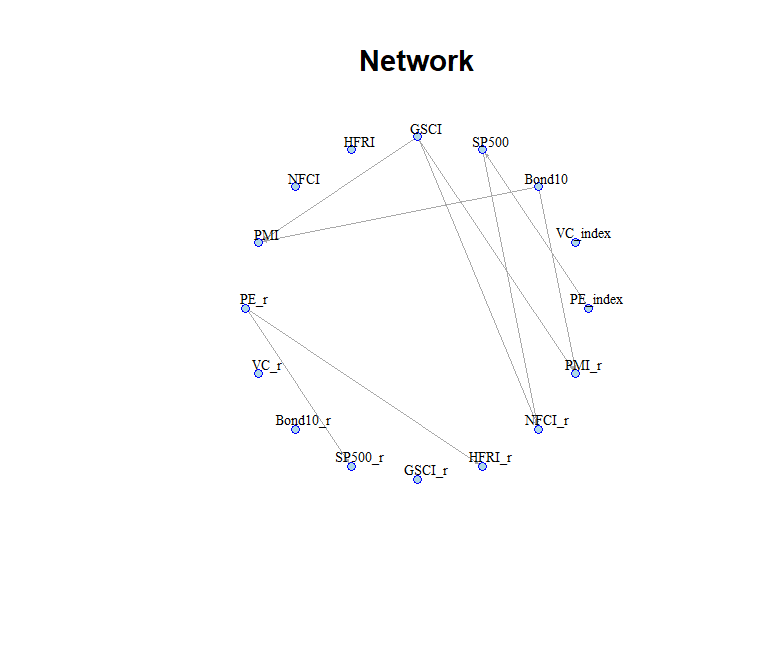
\includegraphics[width=1\linewidth]{Rplot20.png}
    \caption{Individual Pairs}
    \label{fig:enter-label}
\end{figure}
\begin{figure}[H]
    \centering
    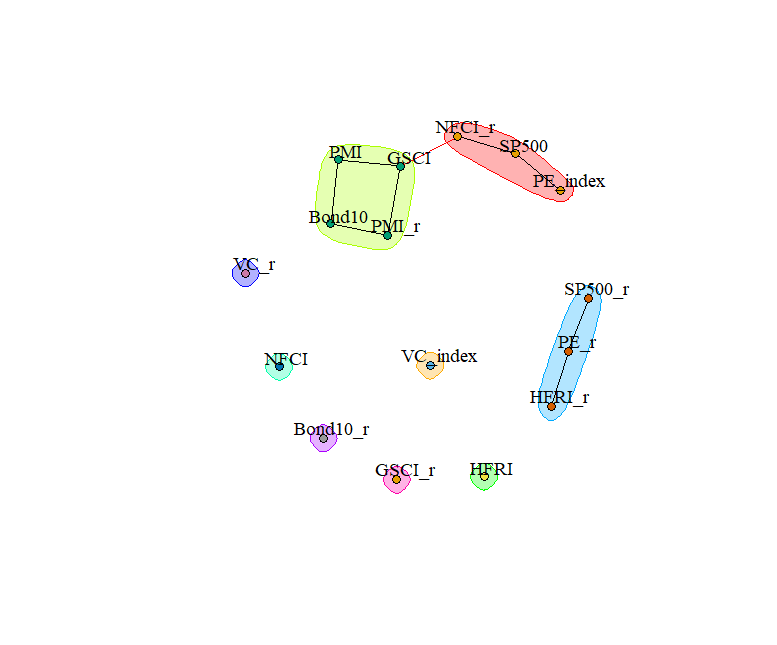
\includegraphics[width=1\linewidth]{Rplot21.png}
    \caption{Individual Pairs}
    \label{fig:enter-label}
\end{figure}
\paragraph{Approach 2: All Bivariate Combinations}
\begin{itemize}

    \item \textbf{Granger Causality Testing}: Perform Granger causality tests for all bivariate combinations and construct the adjacency matrix.
    \item \textbf{Network Visualization}: Visualize the bivariate network without applying multiple testing correction.
\end{itemize}

\begin{figure}[H]
    \centering
    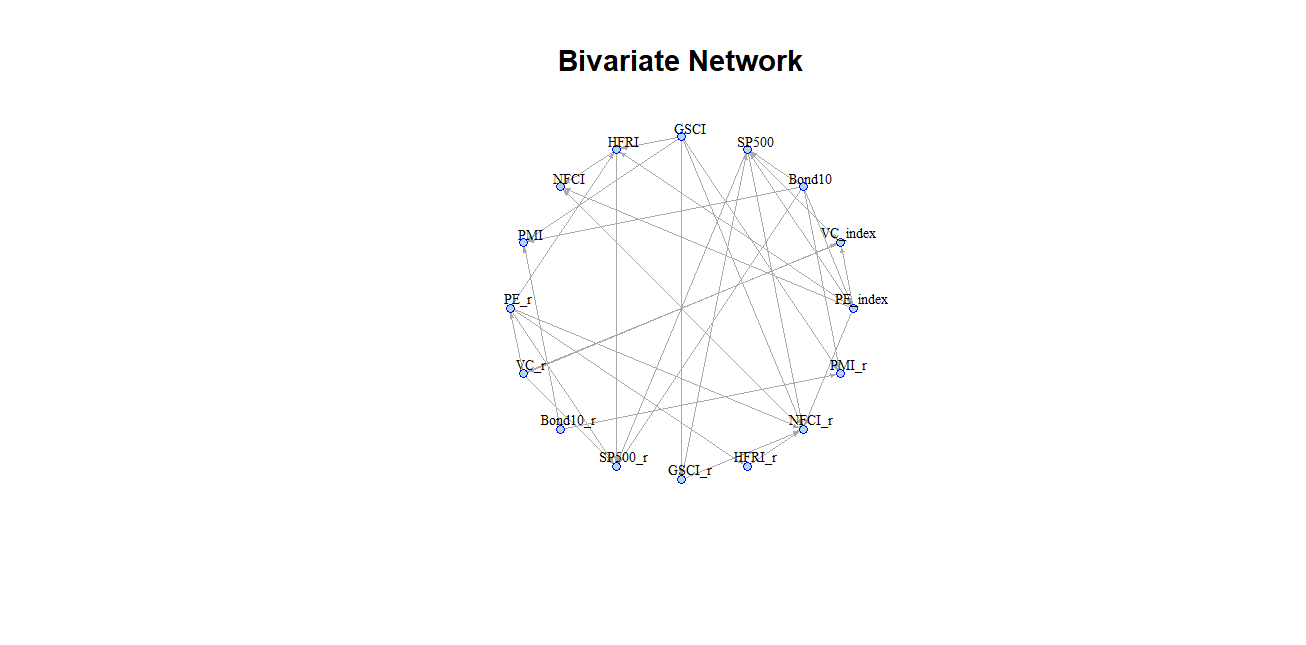
\includegraphics[width=1\linewidth]{Rplot22.png}
    \caption{Bivariate Network}
    \label{fig:enter-label}
\end{figure}
\begin{figure}[H]
    \centering
    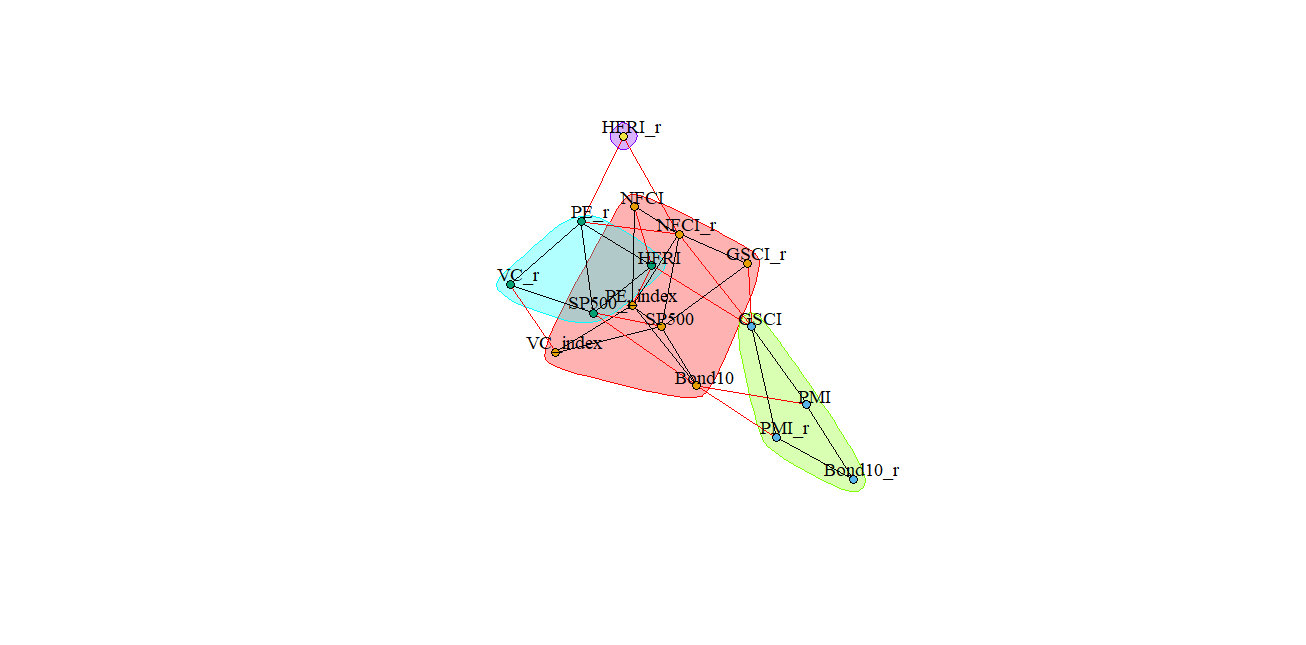
\includegraphics[width=1\linewidth]{Rplot23.png}
    \caption{Bivariate Network}
    \label{fig:enter-label}
\end{figure}

\paragraph{Approach 3: Multiple Combinations}
\begin{itemize}
    \item \textbf{Granger Causality Testing}: Perform Granger causality tests for multiple combinations and construct the adjacency matrix based on significant results.
    \item \textbf{Network Visualization}: Visualize the network for multiple combinations.
\end{itemize}

\begin{figure}[H]
    \centering
    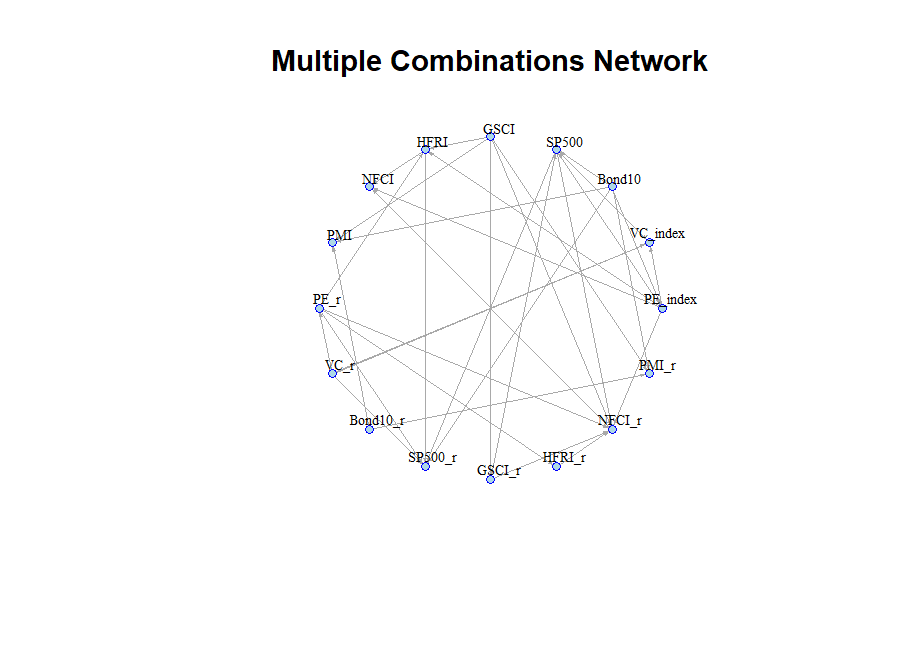
\includegraphics[width=1\linewidth]{Rplot25.png}
    \caption{Multiple Combination Network}
    \label{fig:enter-label}
\end{figure}
\begin{figure}[H]
    \centering
    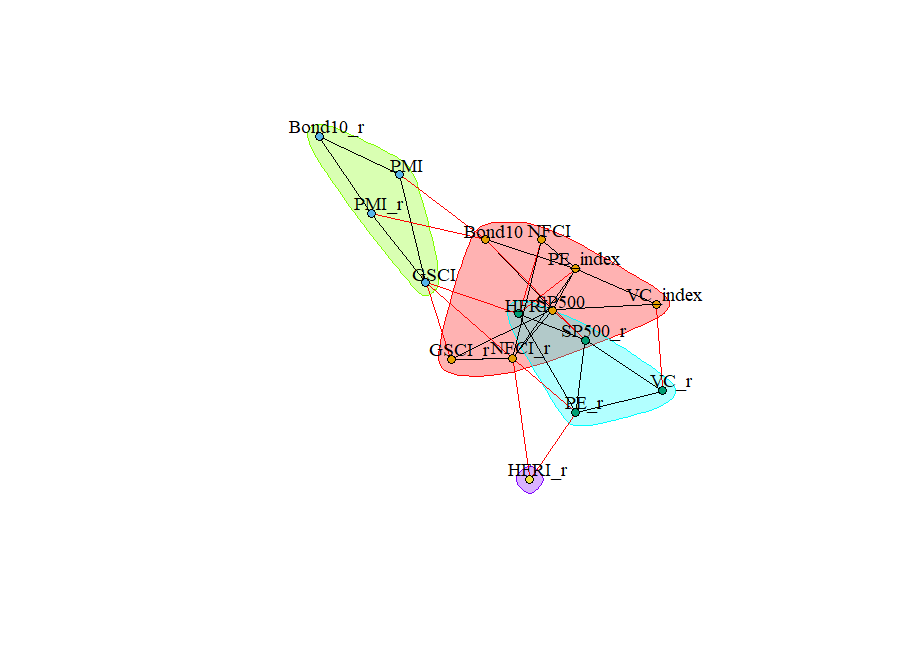
\includegraphics[width=1\linewidth]{Rplot24.png}
    \caption{Multiple Combination Network}
    \label{fig:enter-label}
\end{figure}

The network visualization offers an intuitive understanding of the causal relationship variables. We can determine important influencers and comprehend the directional flow of information within the system by looking at the directed edges.

The robustness of the network is further assessed by performing sensitivity analyses, such as varying the significance level (\(\alpha\)) and the lag length (\(p\)). These analyses help ensure that the identified causal relationships are consistent and reliable.



\subsection{Results}


\section{Empirical applications}





\section{Conclusion}
.
\newpage

\appendix
\section{Technical details}
\subsection{Stationarity and Differencing}

We used the Augmented Dickey-Fuller (ADF) test to check the stationarity of the original time series data and validate the validity of our time series analysis. The ADF test is a popular statistical test for looking for unit roots, which point to non-stationarity in the data.


The ADF test is based on the following regression equation:
\begin{equation} 
\Delta Y_t = \alpha + \beta t + \gamma Y_{t-1} + \delta_1 \Delta Y_{t-1} + \delta_2 \Delta Y_{t-2} + \ldots + \delta_p \Delta Y_{t-p} + \epsilon_t
\end{equation}
where:
\begin{itemize}
    \item \(\Delta\) denotes the first difference operator, i.e., \(\Delta Y_t = Y_t - Y_{t-1}\),
    \item \(\alpha\) is a constant,
    \item \(\beta t\) is a time trend,
    \item \(\gamma\) is the coefficient of the lagged level of the series,
    \item \(\delta_i\) are the coefficients of the lagged first differences,
    \item \(\epsilon_t\) is the white noise error term.
\end{itemize}

The null hypothesis (\(H_0\)) of the ADF test is that the series has a unit root (i.e., the series is non-stationary), which corresponds to \(\gamma = 0\). The alternative hypothesis (\(H_1\)) is that the series is stationary (\(\gamma < 0\)).

The test statistic for the ADF test is given by:
\begin{equation} 
ADF = \frac{\hat{\gamma}}{SE(\hat{\gamma})}
\end{equation}
where \(\hat{\gamma}\) is the estimated coefficient of \(Y_{t-1}\) and \(SE(\hat{\gamma})\) is its standard error. This test statistic is compared against critical values from the Dickey-Fuller distribution to determine whether to reject the null hypothesis.

The ADF test was performed for each series in our dataset. The results indicated that the PE Index, VC Index, Bond10, SP500, GSCI, and HFRI series were non-stationary at the 5\% significance level. Consequently, we applied first-order differencing to these series to achieve stationarity. The differencing transformation is represented as:
\begin{equation} 
Y_t' = Y_t - Y_{t-1}
\end{equation}
where \(Y_t\) represents the original series and \(Y_t'\) represents the differenced series. This transformation effectively removes trends and seasonality, stabilizing the mean of the time series and making it suitable for further analysis.

Specifically, the ADF test results for key non-stationary series are as follows:

\begin{itemize}
    \item \textbf{PE Index}: ADF Statistic = 2.7188, p-value = 0.9991
    \item \textbf{VC Index}: ADF Statistic = 1.4460, p-value = 0.9973
    \item \textbf{Bond10}: ADF Statistic = -1.1435, p-value = 0.6974
    \item \textbf{SP500}: ADF Statistic = 0.8535, p-value = 0.9925
    \item \textbf{GSCI}: ADF Statistic = -2.6771, p-value = 0.0781
    \item \textbf{HFRI}: ADF Statistic = 1.3785, p-value = 0.9970
\end{itemize}

The NFCI, PMI, PE\_r, VC\_r, Bond10\_r, S\&P 500\_r, GSCI\_r, HFRI\_r, NFCI\_r, and PMI\_r series were found to be stationary without the need for differencing.

We employed the \texttt{HDGC\_VAR} function from the HDGCvar methodology, which can handle both stationary and non-stationary data together. This approach is based on the work of A. Hecq, L. Margaritella, and S. Smeekes (2019) in their paper "Granger Causality Testing in High Dimensional VARs: a Post Double Selection Procedure" \cite{Hecq2019}. 

Upon taking the first difference, all our data became stationary, as verified by the plots of the \textit{index\_r} series in the appendix section. This methodology seamlessly integrated stationary and non-stationary series into our analysis.
\subsection{Augmented Dickey-Fuller (ADF) Test Results}

This section presents the detailed results of the Augmented Dickey-Fuller (ADF) test conducted on the original time series data to check for stationarity. The critical values at the 1\%, and 5\%, levels are also included.

\begin{table}[h!]
\centering
\caption{ADF Test Results for Original Series}
\begin{tabular}{|l|c|c|c|c|}
\hline
\textbf{Series} & \textbf{ADF Statistic} & \textbf{p-value} & \textbf{Critical Value (1\%)} & \textbf{Critical Value (5\%)} \\ \hline
PE Index        & 2.7188                 & 0.9991           & -3.4861                      & -2.8859                      \\ \hline
VC Index        & 1.4460                 & 0.9973           & -3.4829                      & -2.8846                      \\ \hline
Bond10          & -1.1435                & 0.6974           & -3.4813                      & -2.8839                      \\ \hline
SP500           & 0.8535                 & 0.9925           & -3.4851                      & -2.8855                      \\ \hline
GSCI            & -2.6771                & 0.0781           & -3.4817                      & -2.8840                      \\ \hline
HFRI            & 1.3785                 & 0.9970           & -3.4856                      & -2.8857                      \\ \hline
NFCI            & -4.1075                & 0.0009           & -3.4813                      & -2.8839                      \\ \hline
PMI             & -5.4408                & 2.78e-06         & -3.4825                      & -2.8844                      \\ \hline
PE Return       & -5.1126                & 1.32e-05         & -3.4825                      & -2.8844                      \\ \hline
VC Return       & -4.7535                & 6.67e-05         & -3.4825                      & -2.8844                      \\ \hline
Bond10 Return   & -10.7399               & 2.84e-19         & -3.4813                      & -2.8839                      \\ \hline
SP500 Return    & -11.2354               & 1.86e-20         & -3.4813                      & -2.8839                      \\ \hline
GSCI Return     & -10.7685               & 2.42e-19         & -3.4813                      & -2.8839                      \\ \hline
HFRI Return     & -9.6586                & 1.37e-16         & -3.4813                      & -2.8839                      \\ \hline
NFCI Return     & -10.6549               & 4.56e-19         & -3.4813                      & -2.8839                      \\ \hline
PMI Return      & -7.0185                & 6.63e-10         & -3.4829                      & -2.8846                      \\ \hline
\end{tabular}
\end{table}

The series identified as non-stationary at the 5\% significance level include PE Index, VC Index, Bond10, SP500, GSCI, and HFRI. The necessary first-order differencing was applied to these series to achieve stationarity, as described in Section \textit{Stationarity and Differencing} of the methodology.




\subsection{High-Dimensional VAR Model Specification}
We use a high-dimensional Vector Autoregressive (HD-VAR) model to capture time series variable characteristics. 

 HD-VAR model:

\begin{equation} 
\mathbf{Y}_t = \Phi_1 \mathbf{Y}_{t-1} + \Phi_2 \mathbf{Y}_{t-2} + \ldots + \Phi_p \mathbf{Y}_{t-p} + \boldsymbol{\epsilon}_t
\end{equation}

where:
\begin{itemize}
    \item \(\mathbf{Y}_t\) is an \(n \times 1\) vector of observations at time \(t\),
    \item \(\Phi_i\) are \(n \times n\) coefficient matrices for each lag \(i\),
    \item \(p\) is the maximum lag order,
    \item \(\boldsymbol{\epsilon}_t\) is an \(n \times 1\) vector of white noise error terms with covariance matrix \(\mathbf{\Sigma}\).
\end{itemize}

\subsubsection{Lag Order Selection}

The optimal lag order \(p\) is determined using the Bayesian Information Criterion (BIC):

\begin{equation} 
\text{BIC}(p) = \log(\hat{\sigma}^2) + \frac{p \log(T)}{T}
\end{equation}

where:
\begin{itemize}
    \item \(\hat{\sigma}^2\) is the estimated variance of the residuals,
    \item \(T\) is the sample size.
\end{itemize}

The BIC is a criterion for model selection among a finite set of models; the model with the lowest BIC is preferred. The BIC penalizes the complexity of the model (i.e., the number of parameters) and thus helps to avoid overfitting.

\subsubsection{High-Dimensional Considerations}

In high-dimensional settings where the number of variables \(n\) can be large relative to the number of observations \(T\), traditional VAR models can suffer from overfitting and multicollinearity. Therefore, it's essential to employ techniques that can handle high-dimensional data effectively.

\subsubsection{Stability and Invertibility Conditions}

For the VAR model to be stable, the roots of the characteristic polynomial must lie outside the unit circle. The characteristic polynomial for the VAR(p) model is given by:

\begin{equation} 
\det(I - \Phi_1 z - \Phi_2 z^2 - \ldots - \Phi_p z^p) \neq 0 \quad \text{for} \quad |z| \leq 1
\end{equation}

If this condition holds, the VAR process is stationary and invertible.

\subsubsection{Estimation Procedure}

Given the high dimensionality of the dataset, we implement a post-double-selection procedure as described by Belloni, Chernozhukov, and Hansen (2014) to ensure the robustness of the model. This procedure involves:

\begin{enumerate}
    \item \textbf{Initial LASSO Regression:} Identify a preliminary set of predictors for each variable in the VAR system by performing LASSO regressions on the dependent variable with all potential predictors.
    \item \textbf{Second Stage Selection:} Refine the set of predictors by performing additional LASSO regressions for each selected predictor on the remaining potential predictors.
    \item \textbf{OLS Estimation:} Use the refined set of predictors to perform Ordinary Least Squares (OLS) estimation, ensuring the final model includes all relevant variables.
\end{enumerate}

\subsubsection{Asymptotic Properties}

To ensure the validity of our HD-VAR model, we rely on the following asymptotic properties:

\paragraph{Consistency}
Under appropriate conditions, including sparsity of the true coefficient vectors and the irrepresentable condition, the LASSO estimator can consistently identify the non-zero coefficients.

\paragraph{Asymptotic Normality}
The distribution of the OLS estimator in the post-double-selection procedure converges to a normal distribution as the sample size \(T\) increases. This allows for valid statistical inference on the estimated coefficients.

\subsubsection{Eigenvalue Conditions}

The eigenvalues of the coefficient matrices \(\Phi_i\) play a crucial role in the stability and invertibility of the VAR model. For the VAR model to be stable, the largest eigenvalue of the companion matrix must be less than one in absolute value. The companion matrix \(\mathbf{C}\) is constructed as follows:

\[
\mathbf{C} = \begin{pmatrix}
\Phi_1 & \Phi_2 & \ldots & \Phi_p \\
\mathbf{I} & \mathbf{0} & \ldots & \mathbf{0} \\
\mathbf{0} & \mathbf{I} & \ldots & \mathbf{0} \\
\vdots & \vdots & \ddots & \vdots \\
\mathbf{0} & \mathbf{0} & \ldots & \mathbf{I}
\end{pmatrix}
\]

where \(\mathbf{I}\) is the identity matrix and \(\mathbf{0}\) is a matrix of zeros.

By ensuring that the absolute values of the eigenvalues of \(\mathbf{C}\) are less than one, we confirm the stability of the VAR model.

\subsubsection{Implementation in R}

The estimation is implemented using the \texttt{glmnet} package in R, which efficiently handles high-dimensional data. The optimal regularization parameter \(\lambda\) is selected via cross-validation, ensuring that the model achieves a balance between bias and variance.

By incorporating these advanced techniques, the HD-VAR model effectively captures the complex interdependencies among the time series variables, providing a robust framework for subsequent Granger causality testing and inference.
\section{Additional Figures}


\begin{figure}[H]
    \centering
    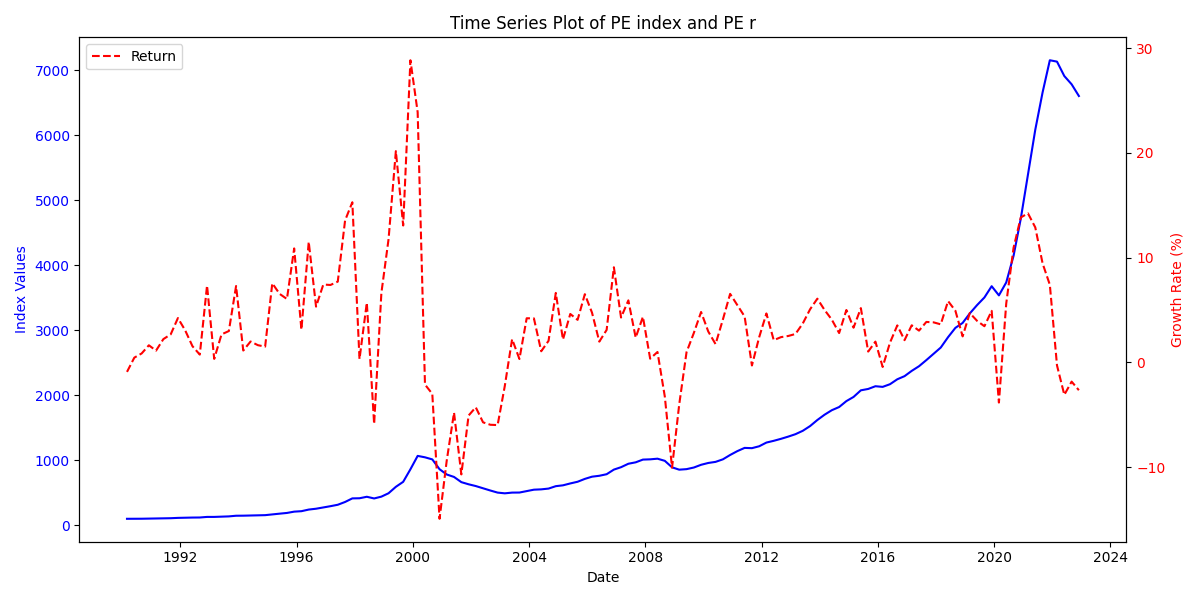
\includegraphics[width=1\linewidth]{plot_PE_index.png}
    \caption{Private Equity (PE) Index.}
    \label{fig:pe_index}
\end{figure}

\begin{figure}[H]
    \centering
    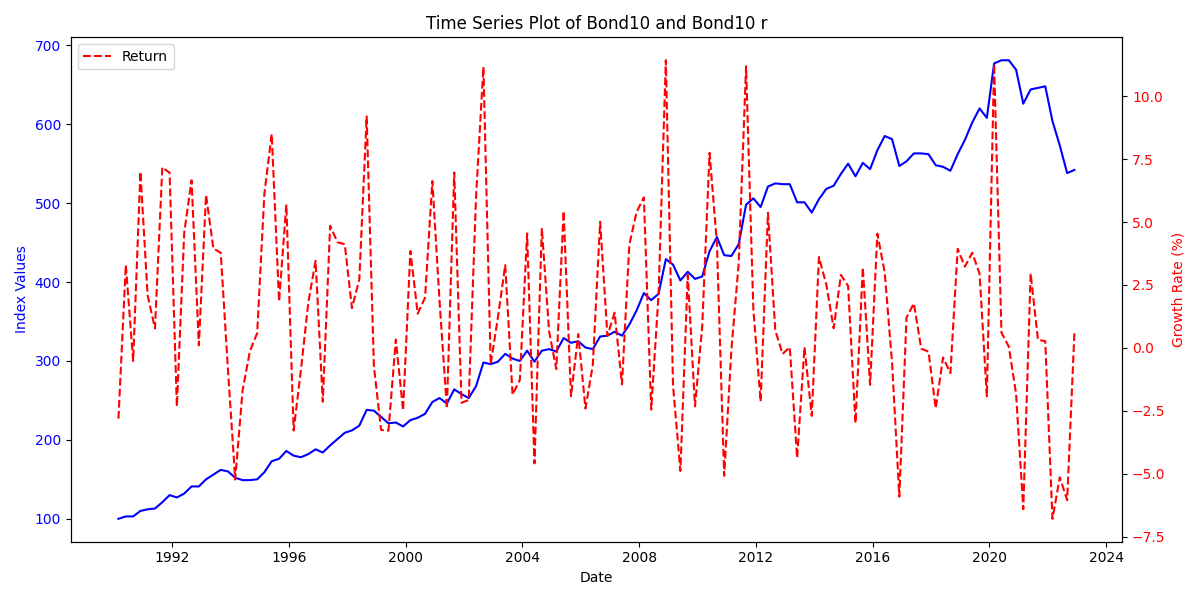
\includegraphics[width=1\linewidth]{plot_Bond10.png}
    \caption{10-Year Government Bond (Bond10).}
    \label{fig:bond10}
\end{figure}

\begin{figure}[H]
    \centering
    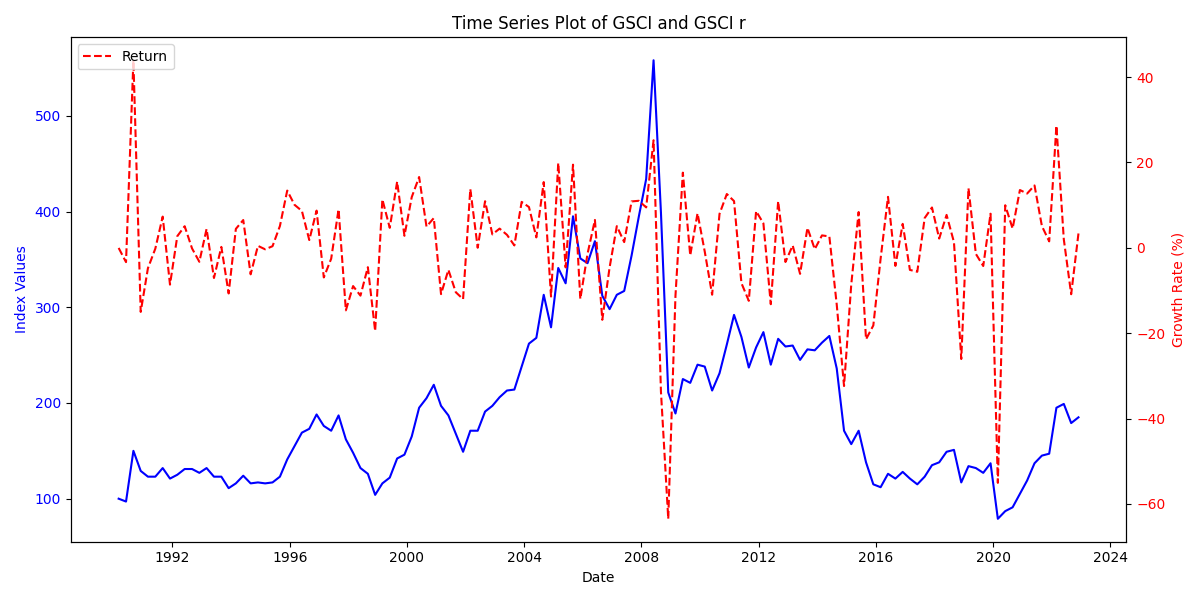
\includegraphics[width=1\linewidth]{plot_GSCI.png}
    \caption{Goldman Sachs Commodity Index (GSCI).}
    \label{fig:gsci}
\end{figure}

\begin{figure}[H]
    \centering
    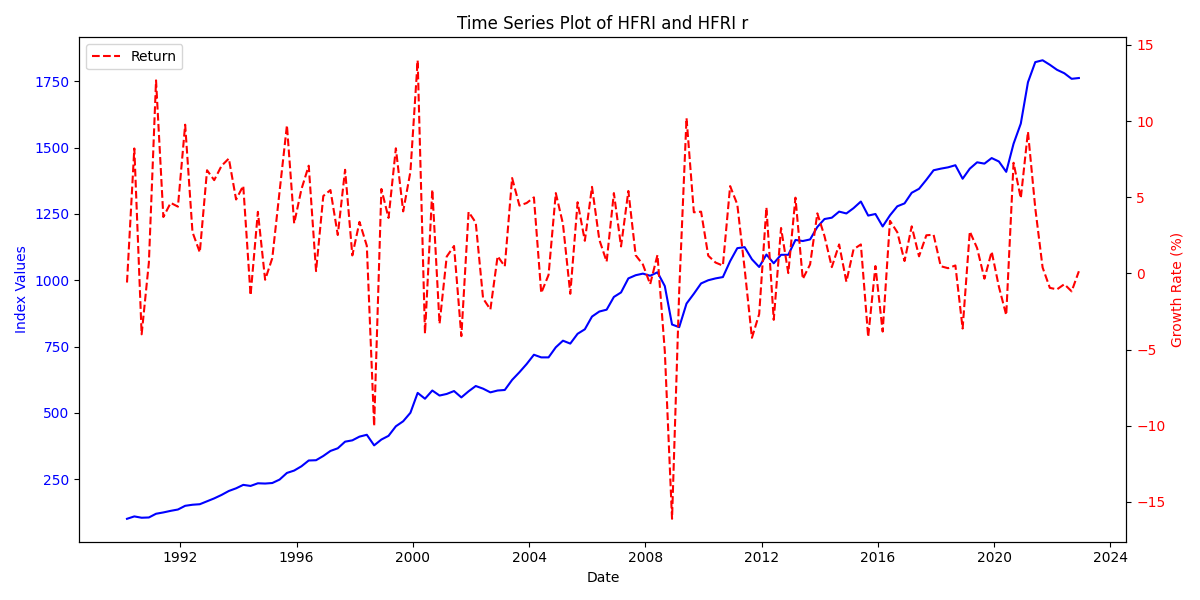
\includegraphics[width=1\linewidth]{plot_HFRI.png}
    \caption{Hedge Fund Research Index (HFRI).}
    \label{fig:hfri}
\end{figure}

\begin{figure}[H]
    \centering
    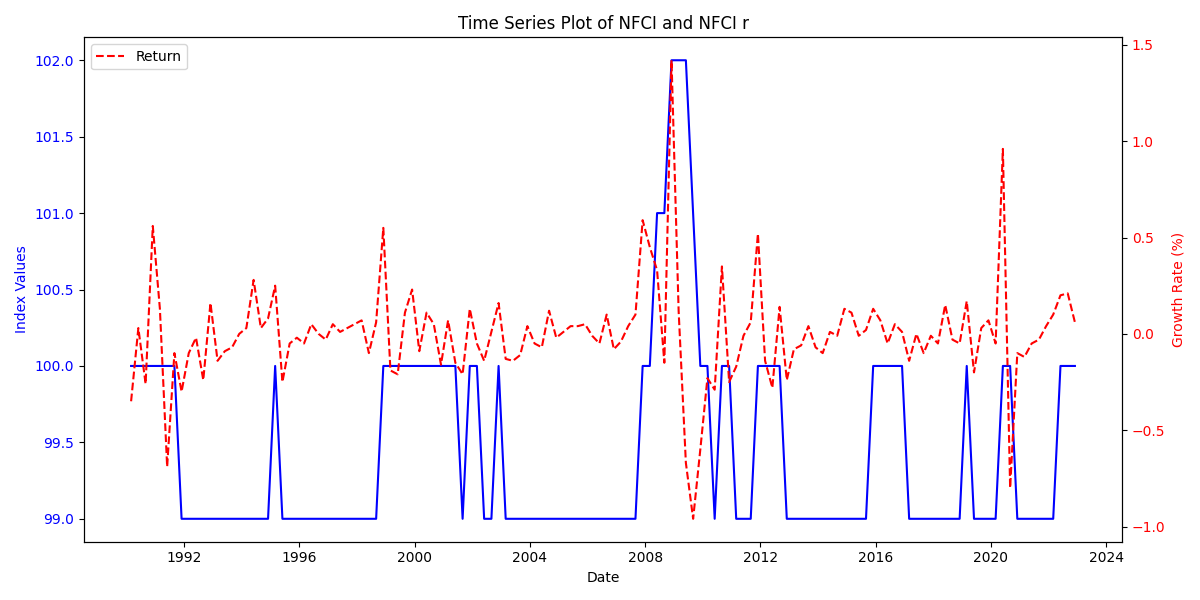
\includegraphics[width=1\linewidth]{plot_NFCI.png}
    \caption{National Financial Conditions Index (NFCI).}
    \label{fig:nfci}
\end{figure}

\begin{figure}[H]
    \centering
    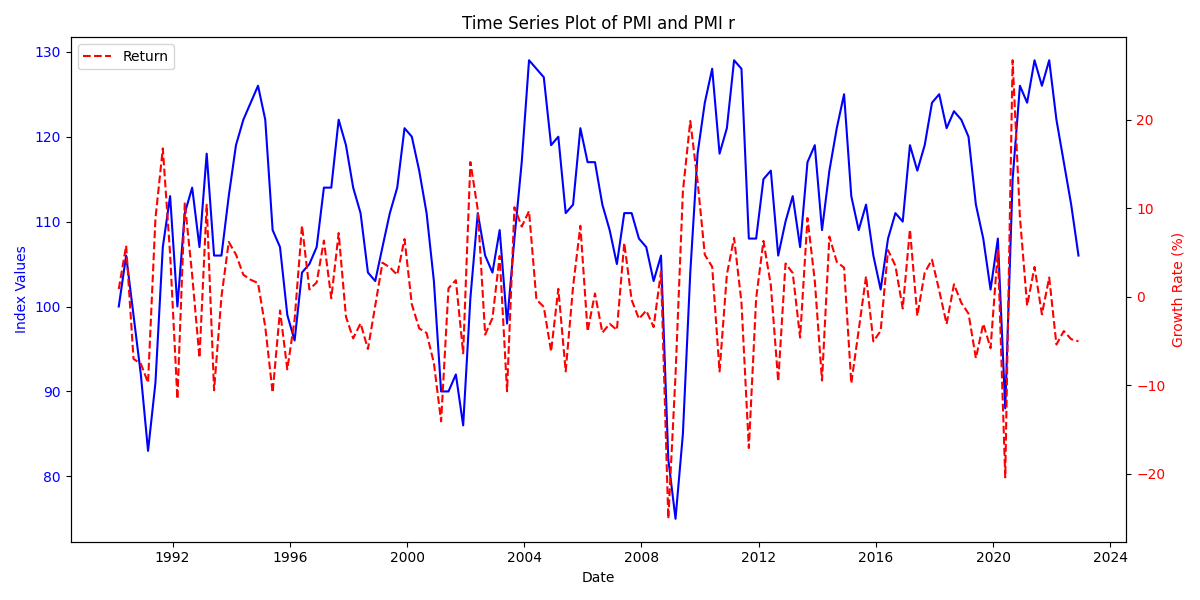
\includegraphics[width=1\linewidth]{plot_PMI.png}
    \caption{Purchasing Managers' Index (PMI).}
    \label{fig:pmi}
\end{figure}

\begin{figure}[H]
    \centering
    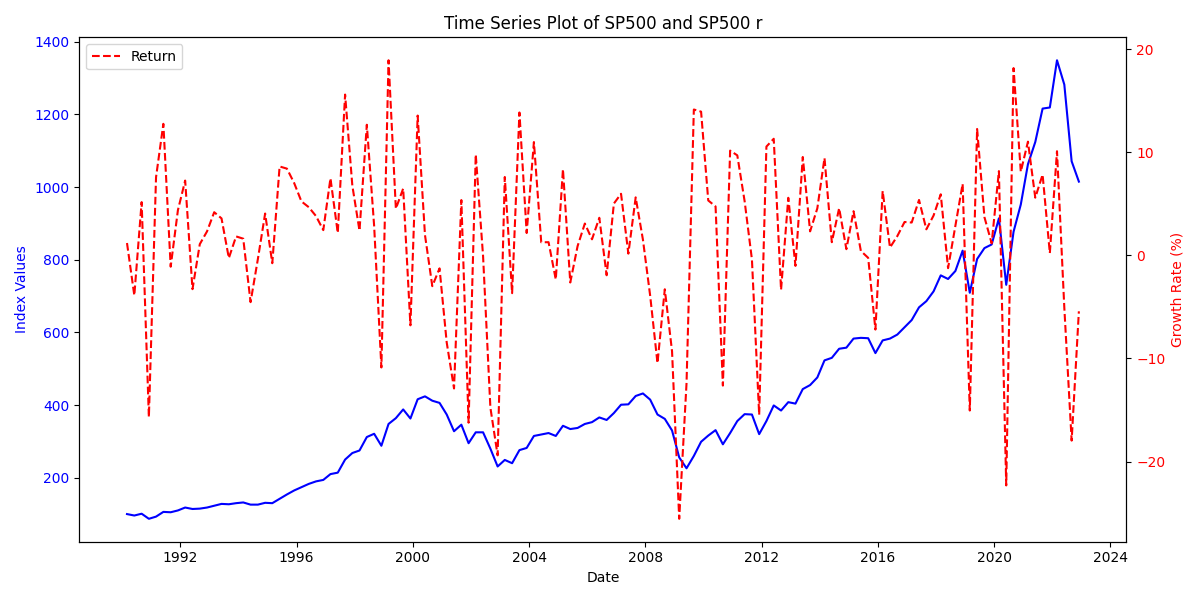
\includegraphics[width=1\linewidth]{plot_SP500.png}
    \caption{S\&P 500 Index (SP500).}
    \label{fig:sp500}
\end{figure}

\begin{figure}[H]
    \centering
    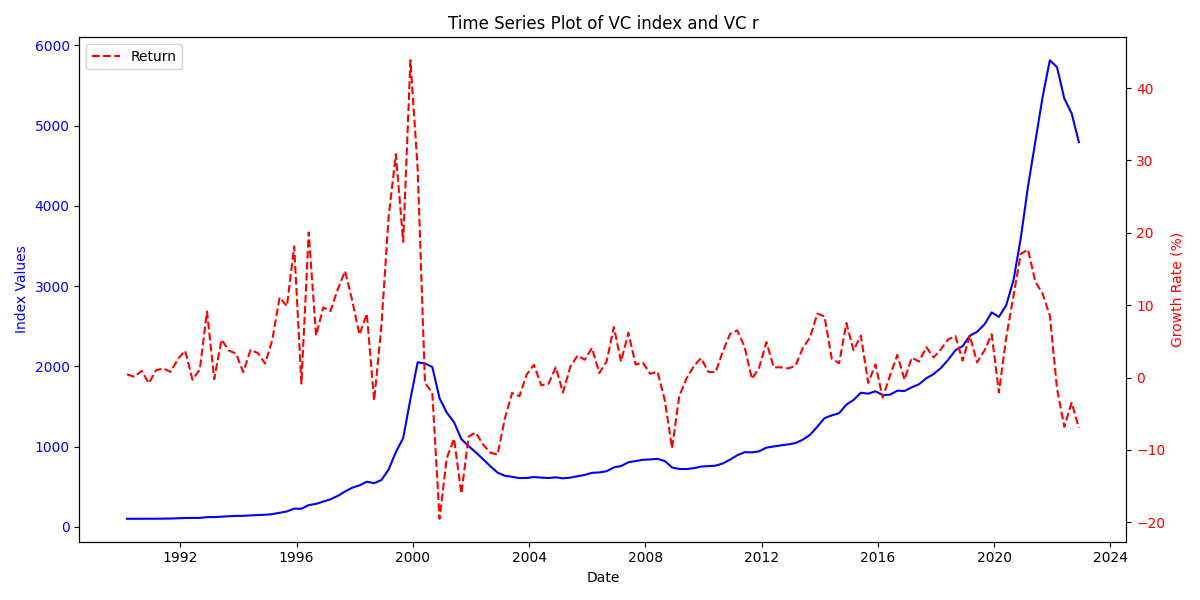
\includegraphics[width=1\linewidth]{plot_VC_index.png}
    \caption{Venture Capital (VC) Index.}
    \label{fig:vc_index}
\end{figure}


\section{Transformed Stationary Series}

This section includes the plots of the series that were non-stationary but made stationary through first-order differencing.

\begin{figure}[H]
    \centering
    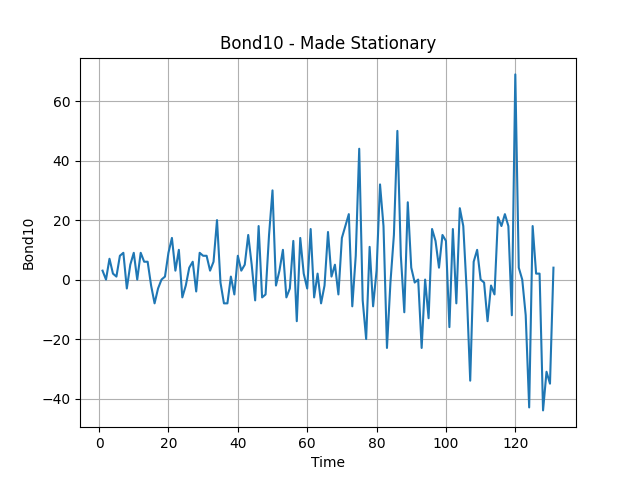
\includegraphics[width=0.75\linewidth]{Bond10_stationary.png}
        \caption{Bond10}
    \label{fig:enter-label}
\end{figure}
\begin{figure}[H]
    \centering
    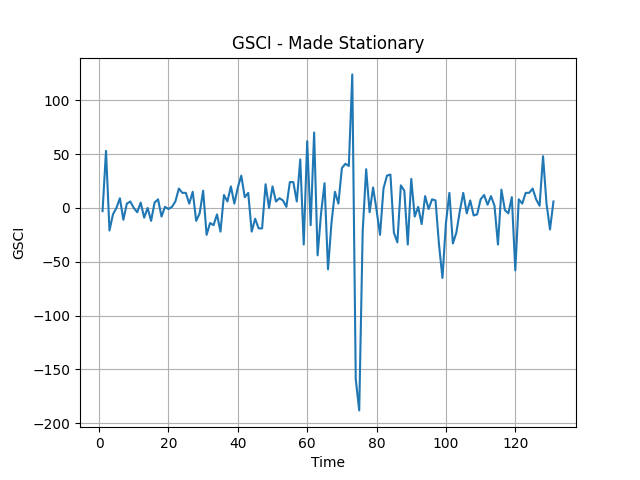
\includegraphics[width=0.75\linewidth]{GSCI_stationary.png}
    \caption{GSCI}
    \label{fig:enter-label}
\end{figure}
\begin{figure}[H]
    \centering
    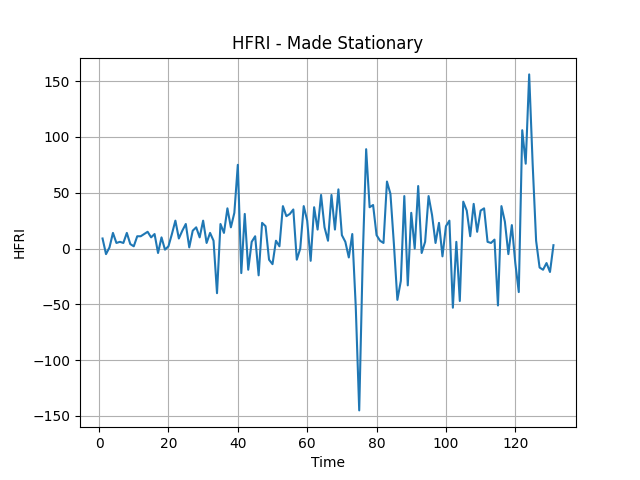
\includegraphics[width=0.75\linewidth]{HFRI_stationary.png}
    \caption{HFRI}
    \label{fig:enter-label}
\end{figure}

\begin{figure}[H]
    \centering
    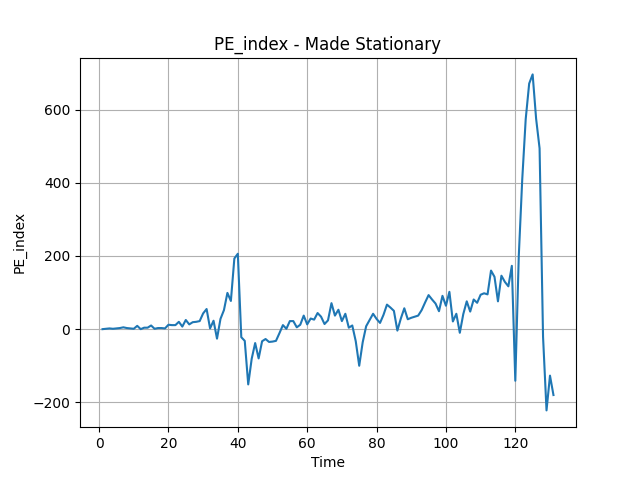
\includegraphics[width=0.75\linewidth]{PE_index_stationary.png}
    \caption{PE INDEX}
    \label{fig:enter-label}
\end{figure}
\begin{figure}[H]
    \centering
    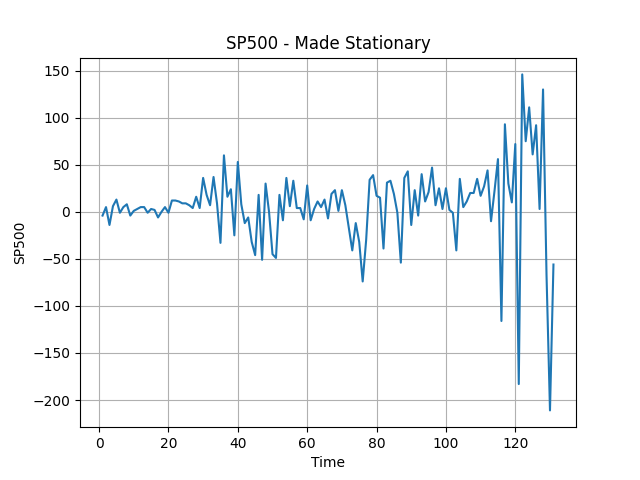
\includegraphics[width=0.75\linewidth]{SP500_stationary.png}
    \caption{S\&P 500}
    \label{fig:enter-label}
\end{figure}
\begin{figure}[H]
    \centering
    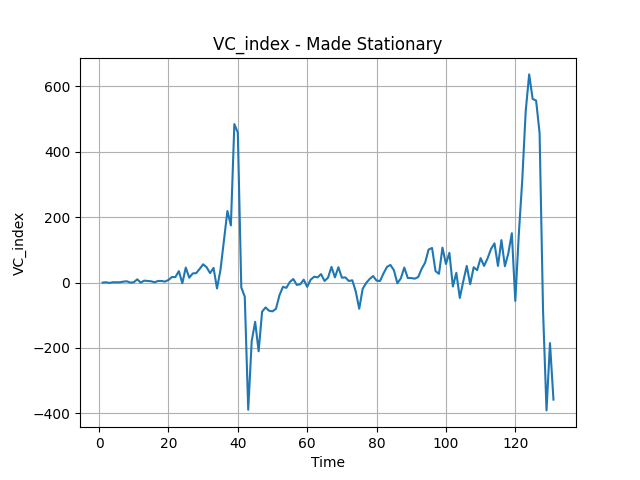
\includegraphics[width=0.75\linewidth]{VC_index_stationary.png}
    \caption{VC INDEX}
    \label{fig:enter-label}
\end{figure}

\section{Normalized Series}
\begin{figure}[H]
    \centering
    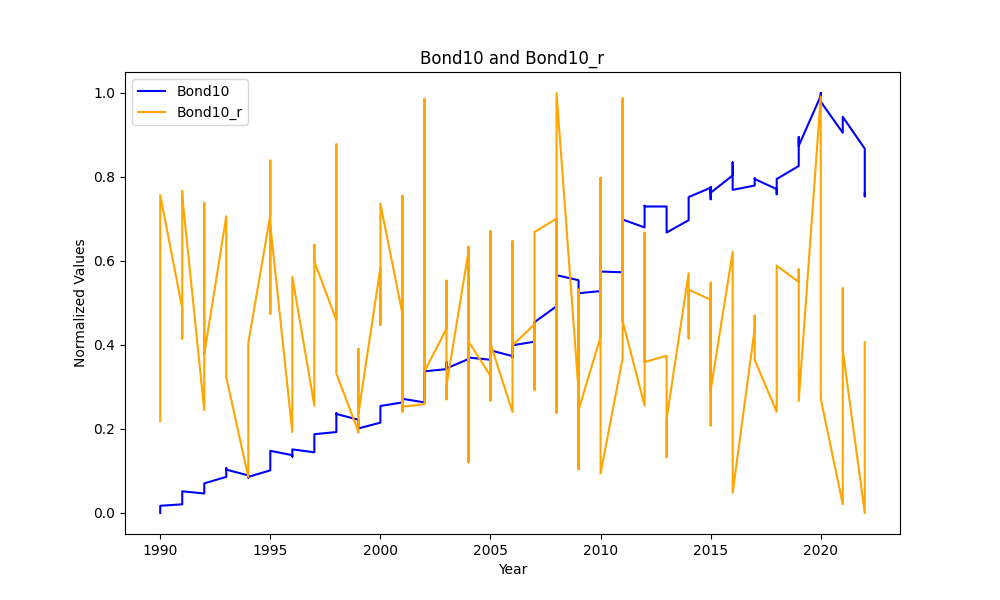
\includegraphics[width=0.75\linewidth]{Bond10_Bond10_r.png}
    \caption{Normalized Bond10 and Bond10 Growth Rate}
    \label{fig:enter-label}
\end{figure}
\begin{figure}[H]
    \centering
    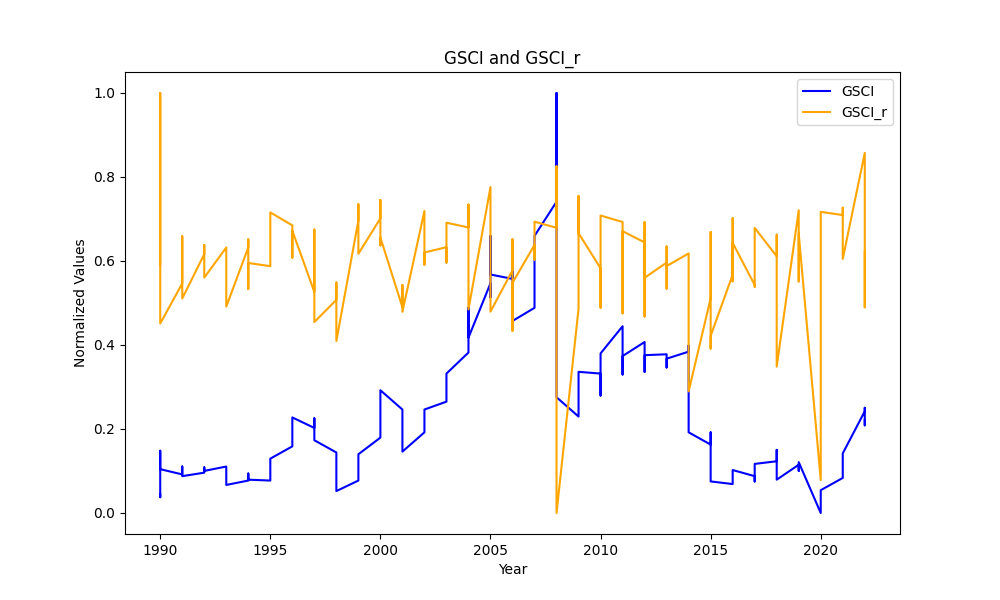
\includegraphics[width=0.75\linewidth]{GSCI_GSCI_r.png}
    \caption{Normalized GSCI and GSCI Growth Rate}
    \label{fig:enter-label}
\end{figure}
\begin{figure}[H]
    \centering
    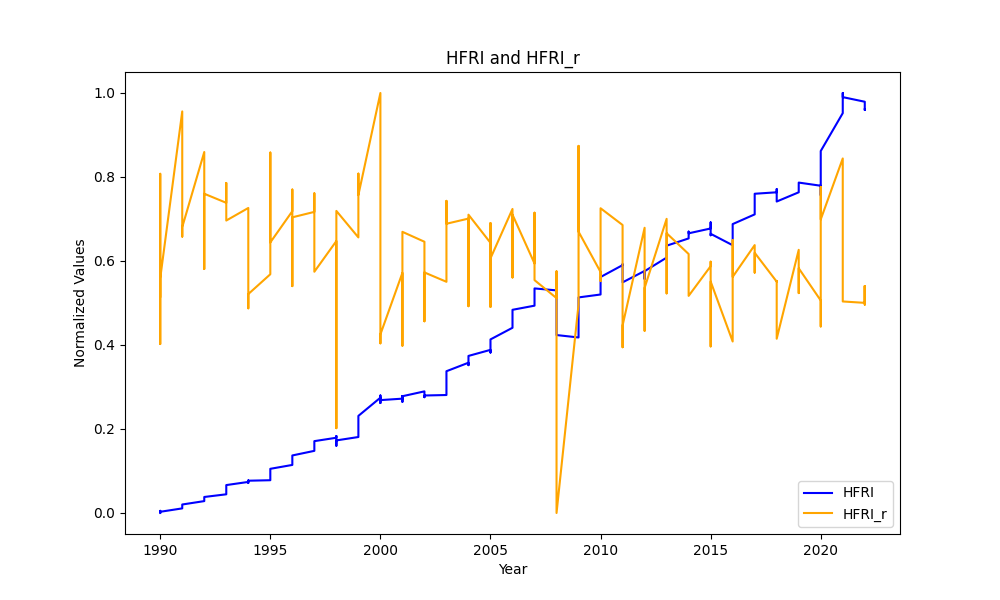
\includegraphics[width=0.75\linewidth]{HFRI_HFRI_r.png}
    \caption{Normalized HFRI and HFRI Growth Rate}
    \label{fig:enter-label}
\end{figure}
\begin{figure}[H]
    \centering
    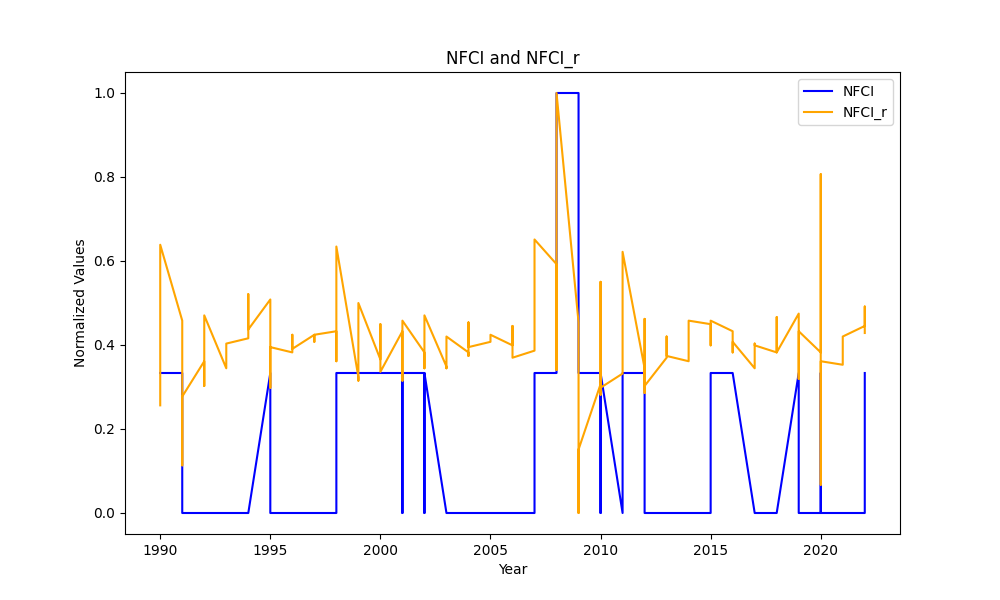
\includegraphics[width=0.75\linewidth]{NFCI_NFCI_r.png}
    \caption{Normalized NFCI and NFCI Growth Rate}
    \label{fig:enter-label}
\end{figure}
\begin{figure}[H]
    \centering
    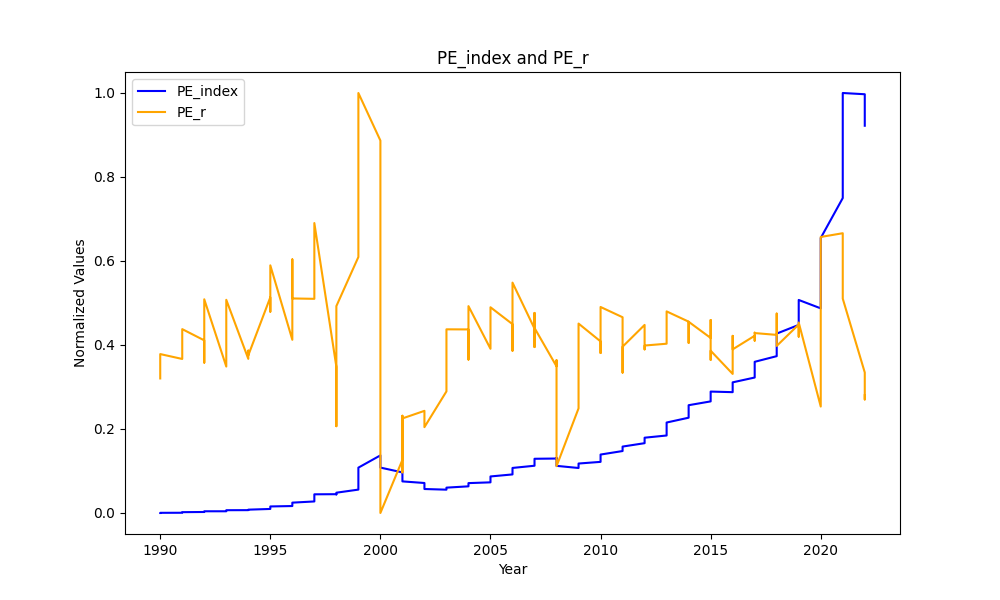
\includegraphics[width=0.75\linewidth]{PE_index_PE_r.png}
    \caption{Normalized PE Index and PE Index Growth Rate}
    \label{fig:enter-label}
\end{figure}
\begin{figure}[H]
    \centering
    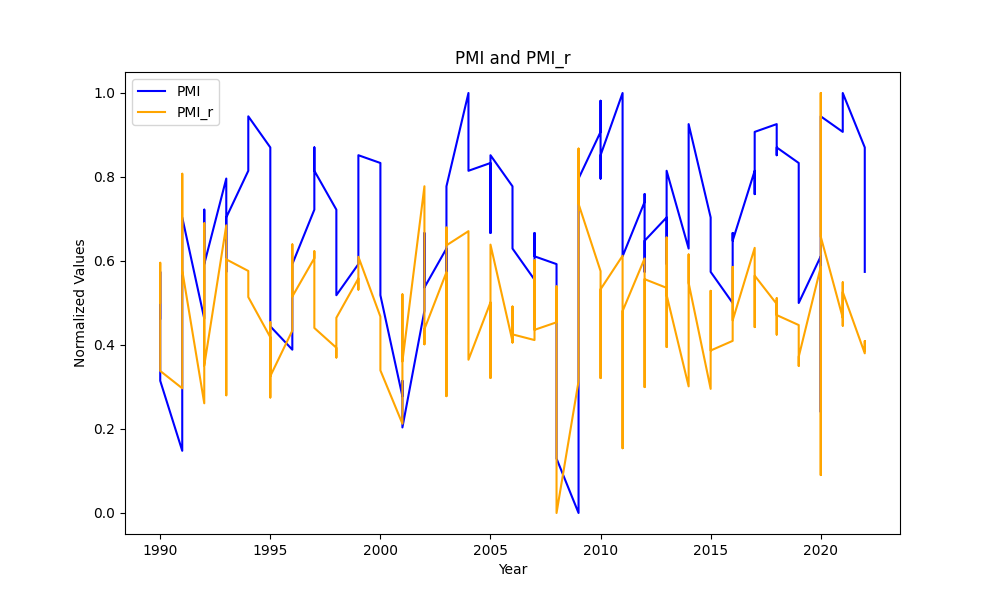
\includegraphics[width=0.75\linewidth]{PMI_PMI_r.png}
    \caption{Normalized PMI and PMI Growth Rate}
    \label{fig:enter-label}
\end{figure}
\begin{figure}[H]
    \centering
    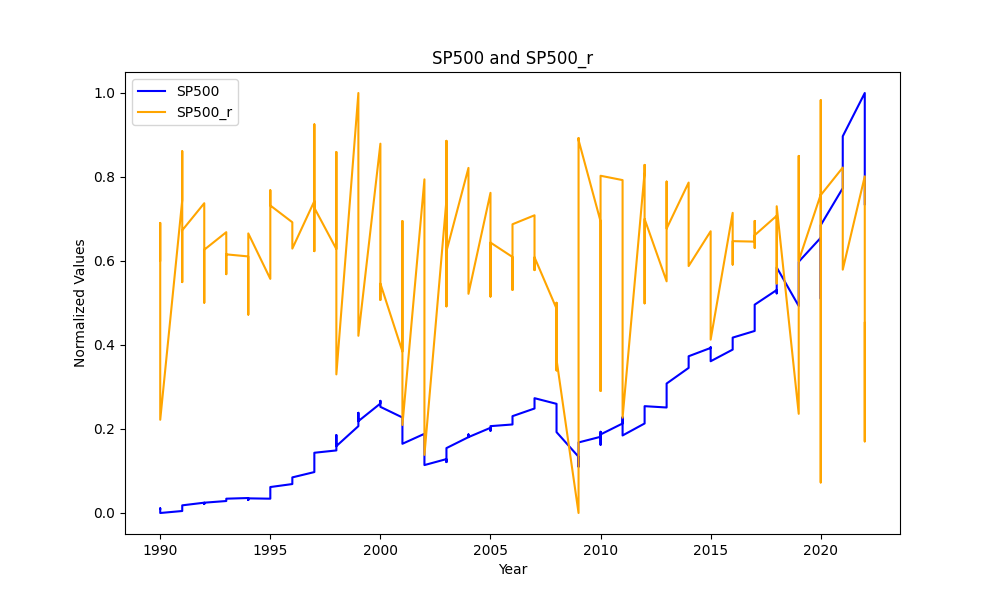
\includegraphics[width=0.75\linewidth]{SP500_SP500_r.png}
    \caption{Normalized S\&P 500 and S\&P 500 Growth Rate}
    \label{fig:enter-label}
\end{figure}
\begin{figure}[H]
    \centering
    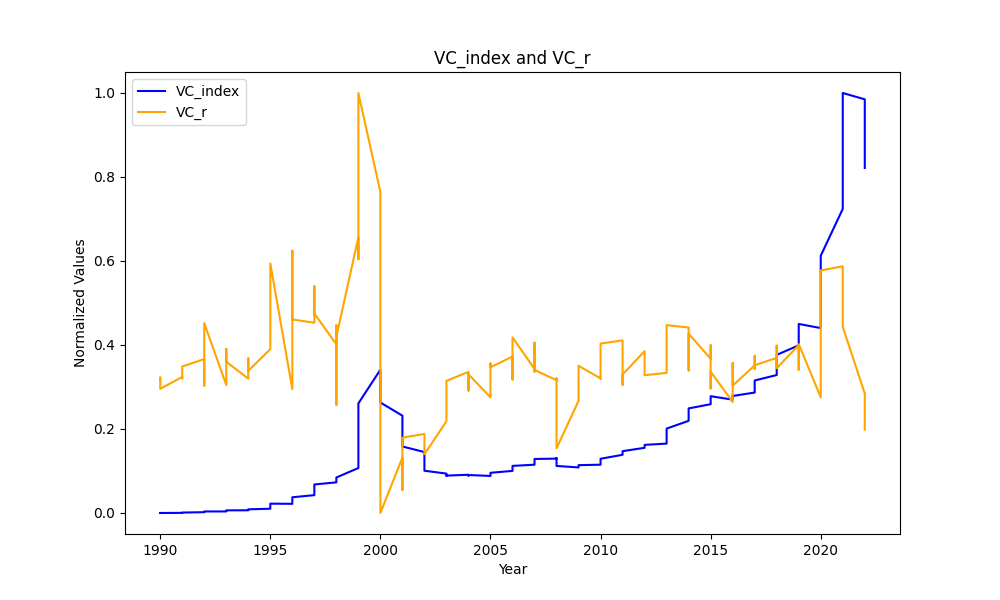
\includegraphics[width=0.75\linewidth]{VC_index_VC_r.png}
    \caption{Normalized VC Index and VC Index Growth Rate}
    \label{fig:enter-label}
\end{figure}

\newpage


\bibliographystyle{plain}
\bibliography{references}
\end{document}
